\section{Prompt Templates}
\label{app:prompts}

SICA uses domain-specific prompt templates for constraint extraction: one for mathematical reasoning (GSM8K, AIME) and one for logical reasoning (ProofWriter, FOLIO). Both share the same system prompt. The LLM is called with temperature $T{=}0.3$, max tokens $1024$, and structured JSON output mode. Up to 6 traces are processed in parallel via thread pooling, with 2 retries on failure (exponential backoff, base 0.5s).

\paragraph{System Prompt.}

\begin{lstlisting}
You are a constraint extraction tool. Output ONLY
valid JSON. Do NOT solve problems, reason about
correctness, or think step-by-step. Extract
constraints from the given trace exactly as stated.
\end{lstlisting}

\paragraph{Mathematical Constraint Extraction (EXTRACTION\_PROMPT).}

Used for GSM8K and AIME datasets. The placeholder \texttt{\{trace\}} is replaced with the reasoning trace at runtime.

\begin{lstlisting}
Extract mathematical constraints from this reasoning
trace as a JSON object.

Rules:
- type: "equation", "inequality", or "predicate"
- expression: human-readable, e.g. "x + y == 14"
- z3_formula: a single comparison expression in
  Python Z3 syntax
- source_step: step number where the constraint
  appears
- Use variable names from the trace

z3_formula MUST follow these rules:
- Allowed operators: ==, !=, <, >, <=, >=, +, -, *,
  /, **, %
- Use individual named variables: a1, a2, a3...
  NOT arrays a[1] or sets A
- Expand all sums explicitly:
  "a1 + a2 + a3 == 55" NOT "sum([a1,a2,a3])"
- NO Python builtins: sum(), len(), max(), min(),
  list(), set(), range(), int()
- Each z3_formula must be exactly ONE comparison
  (==, !=, <, >, <=, >=)
- For multiple values, write separate constraints
  for each

Output ONLY the JSON below, nothing else:
{"constraints": [{"type": "equation",
  "expression": "x + y == 14",
  "z3_formula": "x + y == 14",
  "source_step": 1}],
 "answer": "final_answer",
 "variables": ["x", "y"]}

Trace:
{trace}
\end{lstlisting}

\paragraph{Logical Constraint Extraction (LOGIC\_EXTRACTION\_PROMPT).}

Used for ProofWriter and FOLIO datasets.

\begin{lstlisting}
IMPORTANT: You are an EXTRACTION tool, NOT a problem
solver.
- Do NOT re-solve or re-reason about the problem.
- Do NOT verify whether the trace's reasoning is
  correct.
- ONLY extract the logical constraints that are
  explicitly stated or used in the trace below.
- Output ONLY the JSON object, nothing else.

Extract logical constraints from this reasoning trace
about a logic problem.

The problem has facts (base assertions), rules
(grounded implications), and derived conclusions.
Convert each into a Z3 boolean formula.

Variable naming:
- Unary property: property_entity
  (e.g., kind_anne, red_charlie, round_fiona)
- Binary relation: relation_subject_object
  (e.g., eats_bear_squirrel, likes_lion_cat)
- Use lowercase with underscores only

Constraint types:
- "fact": a given assertion,
  e.g., kind_anne == True
- "rule": a grounded implication over specific
  entities, e.g., Implies(kind_anne, nice_anne)
- "derived": an inferred conclusion from facts +
  rules, e.g., nice_anne == True

Z3 operators:
- Implies(a, b) for if-then rules
- And(a, b, ...) for conjunctive conditions
- Or(a, b, ...) for disjunctive conditions
- Not(a) for negation
- == True / == False for boolean assertions

Output ONLY the JSON below, nothing else:
{"constraints": [{"type": "fact",
  "expression": "kind(anne)",
  "z3_formula": "kind_anne == True",
  "source_step": 1}],
 "answer": "True or False or Unknown",
 "variables": ["kind_anne"]}

Trace:
{trace}
\end{lstlisting}

\paragraph{Output Schema.}

Both prompts produce a JSON object with the following structure:

\begin{lstlisting}
{
  "constraints": [
    {
      "type": "<equation|inequality|predicate>
               or <fact|rule|derived>",
      "expression": "<human-readable description>",
      "z3_formula": "<Z3-compatible expression>",
      "source_step": <integer>
    }
  ],
  "answer": "<final answer string>",
  "variables": ["<var1>", "<var2>", "..."]
}
\end{lstlisting}

The pipeline additionally injects an \texttt{answer\_assertion} constraint per trace (not produced by the LLM):

\begin{lstlisting}
{"type": "answer_assertion",
 "expression": "answer is <ans>",
 "z3_formula": "__sica_answer_<ans> == True",
 "source_step": -1}
\end{lstlisting}

\paragraph{Prompt Selection Logic.}

Domain assignment is determined by dataset: FOLIO and ProofWriter use \textsc{Logic\_Extraction\_Prompt}; GSM8K, AIME, StrategyQA, and ARC-Challenge use \textsc{Extraction\_Prompt}. StrategyQA and ARC-Challenge are assigned to the mathematical prompt because their reasoning structure does not involve formal logic predicates or implications, despite StrategyQA producing boolean answers.


\section{Z3 MaxSAT Evaluation Pseudocode}
\label{app:z3-pseudocode}

Algorithm~\ref{alg:maxsat} describes the Z3 MaxSAT solving procedure. Algorithm~\ref{alg:scorer} describes the source-trace attribution scoring.

Domain constraint variables (e.g., \texttt{x + y == 14}) and answer assertion variables (e.g., \texttt{\_\_sica\_answer\_42 == True}) are logically independent in the Z3 formulation. Discriminative signal arises solely from conflicts among domain constraints: when traces supporting different answers produce mutually contradictory constraints, the solver excludes the lower-weight subset, and the scorer penalizes the corresponding answers.

\begin{algorithm}[h]
\caption{Z3 Weighted Partial MAX-SAT}
\label{alg:maxsat}
\begin{algorithmic}[1]
\Require Deduplicated constraint set $\mathcal{C} = \{(c_m, w_m, S_m)\}_{m=1}^M$ where $c_m$ is a Z3 formula, $w_m$ is weight, $S_m$ is the set of source trace indices
\Ensure Partition $(\mathcal{C}^*, \mathcal{C}^{\setminus})$ where $\mathcal{C}^*$ is the max-weight satisfiable subset
\State $\textit{opt} \gets \textsc{Z3.Optimize()}$
\For{$m = 1, \ldots, M$}
    \State $b_m \gets$ fresh Boolean indicator
    \State $\textit{opt}.\textsc{Add}(b_m \Rightarrow c_m)$ \Comment{soft clause guarded by indicator}
    \State $\textit{opt}.\textsc{AddSoft}(b_m,\; \text{weight}=w_m)$
\EndFor
\State $\textit{result} \gets \textit{opt}.\textsc{Check}()$
\State $\textit{model} \gets \textit{opt}.\textsc{Model}()$
\State $\mathcal{C}^* \gets \{(c_m, w_m, S_m) : \textit{model}(b_m) = \top\}$
\State $\mathcal{C}^{\setminus} \gets \mathcal{C} \setminus \mathcal{C}^*$
\State \Return $(\mathcal{C}^*, \mathcal{C}^{\setminus})$
\end{algorithmic}
\end{algorithm}

\begin{algorithm}[h]
\caption{Source-Trace Attribution Scoring}
\label{alg:scorer}
\begin{algorithmic}[1]
\Require Satisfied set $\mathcal{C}^*$, excluded set $\mathcal{C}^{\setminus}$, candidate answers $\mathcal{A}$, trace-answer mapping $\tau: \text{trace\_idx} \to a$, penalty weight $\alpha$
\Ensure Score $s(a)$ for each $a \in \mathcal{A}$
\For{each $a \in \mathcal{A}$}
    \State $T_a \gets \{i : \tau(i) = a\}$ \Comment{trace indices producing answer $a$}
    \State $\textit{pos}(a) \gets \sum_{(c,w,S) \in \mathcal{C}^*} w \cdot \mathbf{1}[S \cap T_a \neq \emptyset]$
    \State $\textit{neg}(a) \gets \sum_{(c,w,S) \in \mathcal{C}^{\setminus}} w \cdot \mathbf{1}[S \cap T_a \neq \emptyset]$
    \State $s(a) \gets \textit{pos}(a) - \alpha \cdot \textit{neg}(a)$
\EndFor
\State \Return $a^* = \arg\max_{a \in \mathcal{A}} s(a)$
\end{algorithmic}
\end{algorithm}


\section{Capability-Accuracy Constraint Diagnostics}
\label{app:diagnostics}
\label{app:cil}

\paragraph{Conditional Correction Ratio.}
We define the \textit{Conditional Correction Ratio} (CCR) to summarize verifier--generator complementarity:
\begin{equation}
\label{eq:cil}
\text{CCR}(V, G) = \log \frac{P(V \text{ correct} \mid G \text{ wrong})}{P(V \text{ correct} \mid G \text{ correct})}.
\end{equation}
$\text{CCR} > 0$ means $V$ preferentially corrects $G$'s errors; $\text{CCR} < 0$ indicates shared bias. CCR links our findings: (1)~SCB corresponds to $\text{CCR}(\text{self}, G) \approx 0$; (2)~Finding~2 predicts $\text{CCR}(V, G) > 0$ when $V$ is independent and capable.

\paragraph{Empirical CCR across verifier--generator pairs.}
Table~\ref{tab:cil_empirical} reports CCR for eight verifier--generator--dataset conditions, sorted by CCR descending. All three cross-architecture NLI pairs on ProofWriter yield $\text{CCR} > 0$ (verifier preferentially corrects generator errors), while all three same-model SICA conditions yield $\text{CCR} < 0$ (shared bias). CCR correlates with combo gain: Spearman $\rho = 0.839$, 95\% bootstrap CI $[0.338, 0.990]$; LOO-robust (min $p = 0.014$). Four of eight conditions share the DeBERTa verifier, yielding effective $n < 10$; results should be interpreted as a consistent pattern rather than a precise effect size.

\begin{table}[h]
\centering
\small
\caption{Empirical CCR across eight verifier--generator conditions (sorted by CCR descending). $\text{CCR} > 0$: cross-architecture NLI verifiers on ProofWriter. $\text{CCR} < 0$: same-model SICA or mismatched capability gap.}
\label{tab:cil_empirical}
\resizebox{\columnwidth}{!}{%
\begin{tabular}{@{}lllrr@{}}
\toprule
Generator & Verifier & Dataset & CCR & $\Delta$ (pp) \\
\midrule
Mistral-7B & BART-MNLI & PW-600 & $+$1.86 & $+$5.17 \\
Mistral-7B & DeBERTa-MNLI & PW-600 & $+$1.67 & $+$6.67 \\
Mistral-7B & RoBERTa-MNLI & PW-600 & $+$1.42 & $+$4.17 \\
\addlinespace
Qwen2.5-14B & DeBERTa-MNLI & PW-600 & $-$0.21 & $+$0.33 \\
Mistral-7B & DeBERTa-MNLI & FOLIO-204 & $-$0.47 & $+$2.94 \\
\addlinespace
Mistral-7B & SICA & FOLIO-204 & $-$2.93 & $+$3.43 \\
Qwen2.5-14B & SICA & PW-600 & $-$4.21 & $-$2.50 \\
Mistral-7B & SICA & PW-600 & $-$4.61 & $-$2.83 \\
\bottomrule
\end{tabular}}
\end{table}

\paragraph{Per-condition diagnostics.}
Table~\ref{tab:capability_trap} reports per-condition diagnostic metrics referenced in \S\ref{sec:entropy}.

\begin{table}[h]
\centering
\small
\resizebox{\columnwidth}{!}{%
\begin{tabular}{@{}llrrrr@{}}
\toprule
Model & Domain & $C_0$ (\%) & Extr.\ Rate & Contr.\ Rate & $\Delta$ (pp) \\
\midrule
Qwen2.5-14B & FOLIO & 35.3 & 0.89 & 0.022 & 0.00 \\
Qwen2.5-14B & ProofWriter & 39.2 & 0.89 & 0.022 & $+$0.33 \\
Qwen2.5-14B & StrategyQA$^\dagger$ & 10.0 & 0.70 & --- & $+$3.33 \\
Qwen2.5-14B & ARC-Chall.$^\dagger$ & 5.0 & 1.00 & --- & $-$1.67 \\
Qwen2.5-7B & FOLIO+PW$^\dagger$ & 42.1 & 0.94 & 0.027 & 0.00 \\
Mistral-7B & FOLIO+PW$^\dagger$ & 50.0 & 0.88 & 0.056 & 0.00 \\
LLaMA-3.1-8B & StrategyQA & 41.0 & --- & --- & $+$2.00 \\
LLaMA-3.1-8B & FOLIO & 61.8 & 0.94 & 0.062 & $-$4.41 \\
DeepSeek-R1-7B & FOLIO+PW$^\dagger$ & 58.3 & 0.84 & 0.037 & $-$3.33 \\
QwQ-32B & Combined$^\dagger$ & 2.6 & --- & --- & 0.00 \\
Qwen2.5-14B & GSM8K$^\dagger$ & 13.3 & 0.15 & --- & 0.00 \\
\bottomrule
\end{tabular}}
\caption{Capability-accuracy constraint diagnostics. $C_0$: fraction of questions with multiple distinct candidate answers across $K=12$ traces. Extraction rate: fraction of traces yielding at least one parseable logical constraint. Contradiction rate: fraction of extracted constraint sets with internal contradictions. $\Delta$: SICA$-$SC gap (pp). $\dagger$: $n \leq 60$. Dashes indicate conditions where extraction diagnostics were not computed (StrategyQA uses boolean answers without symbolic extraction; QwQ-32B Combined had near-zero $C_0$, making extraction analysis uninformative). This table includes additional exploratory conditions not reported in Table~\ref{tab:main_results}.}
\label{tab:capability_trap}
\end{table}


\section{Statistical Power Analysis}
\label{app:power}

We compute the minimum detectable effect (MDE) for each condition at $\alpha = 0.05$ and 80\% power using exact binomial power calculations over McNemar discordant pairs. Table~\ref{tab:power} reports three grouped conditions with $n \geq 200$ (Qwen2.5-14B FOLIO and ProofWriter are pooled into a single $n{=}804$ analysis, corresponding to four Table~\ref{tab:main_results} rows), which constitute our confirmatory analyses. The remaining seven conditions ($n \leq 60$) yield infinite MDE due to insufficient discordant pairs and serve only as regime characterization.

\begin{table}[h]
\centering
\small
\resizebox{\columnwidth}{!}{%
\begin{tabular}{lrrrrr}
\toprule
\textbf{Condition} & $n$ & \textbf{MDE} & \textbf{Obs.\ $\Delta$} & \textbf{Obs.\ Pow.} \\
\midrule
Qwen-14B FOLIO+PW   & 804 & 1.86pp & $+$0.25pp & 5.7\%  \\
LLaMA-8B StrategyQA  & 200 & 4.64pp & $+$2.00pp & 20.6\% \\
LLaMA-8B FOLIO       & 204 & 4.84pp & $-$4.41pp & 18.6\% \\
\bottomrule
\end{tabular}}
\caption{Power analysis for confirmatory conditions ($n \geq 200$). MDE = minimum detectable effect at 80\% power. All observed effects fall below their respective MDEs, and observed power remains below 21\% in every case.}
\label{tab:power}
\end{table}

The largest study (Qwen-14B, $n{=}804$, 30 discordant pairs) can detect effects as small as 1.86pp, yet the observed $\Delta$ of $+$0.25pp is an order of magnitude smaller. The two LLaMA-8B conditions require effects of 4.64pp and 4.84pp to reach significance; neither observed $\Delta$ approaches these thresholds. All three conditions are consistent with the null hypothesis that SICA provides no accuracy gain over self-consistency.


\section{Bootstrap Confidence Intervals}
\label{app:bootstrap}

We compute 95\% confidence intervals for $\Delta(\text{SICA} - \text{SC})$ via 10{,}000 bootstrap resamples (percentile method, seed 42). Table~\ref{tab:bootstrap} reports the results for the three confirmatory conditions.

\begin{table}[h]
\centering
\small
\resizebox{\columnwidth}{!}{%
\begin{tabular}{lrrl}
\toprule
\textbf{Condition} & $n$ & \textbf{Obs.\ $\Delta$} & \textbf{95\% CI} \\
\midrule
Qwen-14B FOLIO+PW   & 804 & $+$0.25pp & [$-$1.12, $+$1.62] \\
LLaMA-8B StrategyQA  & 200 & $+$2.00pp & [$-$1.50, $+$5.50] \\
LLaMA-8B FOLIO       & 204 & $-$4.41pp & [$-$5.88, $+$0.98] \\
\bottomrule
\end{tabular}}
\caption{Bootstrap 95\% confidence intervals for $\Delta(\text{SICA} - \text{SC})$ in percentage points. All intervals include zero, consistent with no reliable accuracy difference.}
\label{tab:bootstrap}
\end{table}

All three intervals contain zero. The narrowest interval (Qwen-14B, [$-$1.12, $+$1.62]) rules out practically meaningful gains ($>$2pp) even in the most favorable case. The widest interval (LLaMA-8B FOLIO, [$-$5.88, $+$0.98]) skews negative, indicating that SICA may slightly hurt accuracy in this condition. These results corroborate the McNemar tests and power analysis: no condition provides evidence that logical constraint aggregation improves over majority voting.


\section{Case Studies: Discordant Predictions}
\label{app:case-studies}

Among 804 problems, SICA and SC agree on 773 (96.1\%). The 31 discordant cases comprise 16 SICA wins (SICA correct, SC wrong), 14 SC wins (SC correct, SICA wrong), and 1 where both select different wrong answers. All 31 occur at exact ties (entropy${=}1.0$, 6:6 vote split) or near-ties (entropy${\geq}0.9183$, 8:4 at most), since SICA can differ from SC only when constraint weights shift the majority away from SC's tiebreak choice. We present three representative cases that illustrate the mechanism behind capability-accuracy constraint failures.

\paragraph{Case 1: SICA Wins (folio\_134, FOLIO).}

\emph{Premises}: Some mammals have teeth. Platypus have no teeth. Platypus are mammals. Humans have teeth. \emph{Conclusion}: Humans are mammals. \emph{Gold}: Unknown.

The premises state that \emph{some} mammals have teeth and that humans have teeth, but ``having teeth'' is not sufficient for ``being a mammal'' under open-world semantics. SC produces a 6:6 split (Unknown:6, True:6) and tiebreaks alphabetically to True (wrong). SICA extracts 7 constraints; MaxSAT excludes 1 constraint inconsistent with the rest, reducing the weighted score for True-voting traces and tipping the aggregation to Unknown (correct). The excluded constraint likely captured an incorrect inference step (e.g., affirming the consequent) present only in True-voting traces. While SICA succeeds here, the success is coincidental: the excluded constraint happens to anti-correlate with the correct answer.

\paragraph{Case 2: SC Wins (ProofWriter-1066\_Q6, ProofWriter).}

\emph{Key chain}: White(Bob)$\to$Round(Bob) [white things are round] $\to$ Young(Bob) [all round things are young]. \emph{Conclusion}: ``Bob is not young.'' \emph{Gold}: False (Bob IS young).

SC produces a 6:6 split (False:6, True:6) and tiebreaks to False (correct). SICA extracts 17 constraints; MaxSAT excludes 2 that appear preferentially in False-voting traces. These excluded constraints likely captured correct intermediate derivations (e.g., \texttt{young\_bob == True}) that appeared only in traces completing the full deduction chain. By excluding them, MaxSAT removes evidence supporting the correct answer. SICA selects True (wrong). This case illustrates how self-extracted constraints can systematically mislead: correct reasoning steps become discriminative signals that the solver mistakenly penalizes.

\paragraph{Case 3: Non-discriminative Constraints (ProofWriter-903\_Q6, ProofWriter).}

\emph{Key chain}: Nice(Mouse)$\to$Cold(Mouse) [all nice people are cold] $\to$ Chases(Mouse,Mouse) [nice and cold $\to$ chase mouse]. \emph{Conclusion}: ``The mouse does not chase the mouse.'' \emph{Gold}: False.

SC produces a 6:6 split (False:6, Unknown:6) and tiebreaks to False (correct). SICA extracts 44 constraints but excludes only 1 (2.3\%). The remaining 43 are domain facts and grounded rules (\texttt{nice\_mouse == True}, \texttt{Implies(nice\_mouse, cold\_mouse)}, etc.) that Z3 satisfies identically regardless of the final answer. Both False-voting and Unknown-voting traces share the same premises and grounded rules; they differ only in whether the trace completed the full derivation chain. The single excluded constraint carries negligible weight against 43 shared constraints, so SICA collapses to SC.

\paragraph{Pattern.}

These cases exemplify the general pattern across the 773 agreeing problems: the vast majority of extracted constraints encode shared domain structure rather than answer-specific reasoning, and MaxSAT aggregation degenerates to majority vote. Table~\ref{tab:case_summary} summarizes.

\begin{table}[h]
\centering
\small
\caption{Summary of three representative discordant cases. All occur at exact 6:6 vote ties. Constraint exclusion can break ties in either direction (Cases 1--2) or have no effect (Case 3).}
\label{tab:case_summary}
\resizebox{\columnwidth}{!}{%
\begin{tabular}{@{}lllcccc@{}}
\toprule
Case & ID & Gold & SC & SICA & \#Constr. & Excl.\ (\%) \\
\midrule
1 (SICA win) & folio\_134 & Unknown & True $\times$ & Unknown $\checkmark$ & 7 & 1 (14.3\%) \\
2 (SC win) & PW-1066\_Q6 & False & False $\checkmark$ & True $\times$ & 17 & 2 (11.8\%) \\
3 (Non-disc.) & PW-903\_Q6 & False & False $\checkmark$ & False $\checkmark$ & 44 & 1 (2.3\%) \\
\bottomrule
\end{tabular}}
\end{table}


\section{Oracle Control}
\label{app:oracle}
\label{sec:oracle}
\label{app:pw-oracle-subtype}

Replacing self-extracted constraints with gold annotations (FOLIO logical formulae, ProofWriter DSL), Oracle-SICA yields $+29.90$\,pp on Mistral-7B FOLIO ($p < 10^{-13}$), $+13.73$\,pp on Qwen2.5-14B FOLIO ($p = 2.0 \times 10^{-7}$), and $+17.17$\,pp on ProofWriter ($p < 10^{-14}$). Z3 agrees with gold labels on 95.1\% (FOLIO) and 97.1\% (ProofWriter). The MAX-SAT mechanism is sound; Mistral-7B's best self-extracted $\Delta$ ($+3.43$\,pp) captures only 11.5\% of its oracle ceiling. For Qwen2.5-14B on ProofWriter, the gap is wider still: self-extraction degrades accuracy ($-2.50$\,pp) against an oracle ceiling of $+17.17$\,pp, indicating that stronger models do not self-extract more effectively.

\paragraph{ProofWriter per-subtype analysis.} ProofWriter problems encode deductive rules as Domain-Specific Language (DSL) logic programs. Each problem uses one of four predicate subtypes: attribute predicates with or without negation (AttNeg, AttNoneg), and relation predicates with or without negation (RelNeg, RelNoneg). Relation predicates involve binary relations between entities (e.g., \texttt{eats(bear, squirrel)}), while attribute predicates assign unary properties (e.g., \texttt{kind(anne)}).

The oracle pipeline parses these DSL annotations deterministically into Z3 formulas without any LLM involvement. Of the 600 ProofWriter problems, 594 (99.0\%) produce valid Z3 parses; the remaining 6 fail due to unsupported DSL constructs. Across all 7{,}128 trace-problem pairs submitted to Z3, the solver returns a result in every case (0\% solver errors). Z3 evaluations agree with ground-truth labels on 577 of 594 parseable problems (97.14\%), confirming that the deterministic DSL-to-Z3 translation faithfully preserves problem semantics.

Table~\ref{tab:pw_oracle_subtype} reports the per-subtype breakdown. Relation-predicate subtypes show substantially larger gains than attribute-predicate subtypes: RelNeg improves by $+28.58$~pp and RelNoneg by $+23.29$~pp, compared to $+10.00$~pp for AttNeg and $+8.44$~pp for AttNoneg. Relation predicates involve longer reasoning chains with more intermediate entities, producing greater answer diversity across traces ($C_0$) and more opportunities for oracle constraints to correct errors.

\begin{table}[h]
\centering
\caption{ProofWriter oracle experiment per-subtype breakdown. Oracle-SICA uses gold DSL annotations parsed deterministically to Z3 for consistency checking. Relation-predicate subtypes (RelNeg, RelNoneg) show larger gains than attribute-predicate subtypes; relation subtypes involve longer reasoning chains and benefit more from oracle constraints. Bold indicates best accuracy per row.}
\label{tab:pw_oracle_subtype}
\resizebox{\columnwidth}{!}{%
\begin{tabular}{lcccc}
\toprule
Subtype & $n$ & SC Acc (\%) & Oracle Acc (\%) & $\Delta$ (pp) \\
\midrule
AttNoneg & 154 & 90.26 & \textbf{98.70} & +8.44 \\
AttNeg & 160 & 81.88 & \textbf{91.88} & +10.00 \\
RelNoneg & 146 & 60.96 & \textbf{84.25} & +23.29 \\
RelNeg & 140 & 60.71 & \textbf{89.29} & +28.58 \\
\midrule
Overall & 600 & 74.00 & \textbf{91.17} & +17.17 \\
\bottomrule
\end{tabular}}
\end{table}


\section{Constraint Ablation Details}
\label{app:ablation}
\label{sec:ablation}

\begin{table}[h]
\centering
\small
\caption{Constraint ablation (Qwen2.5-14B, $n = 804$). Agreement: predictions identical to SC. MAX-SAT and count-only produce nearly identical predictions, confirming that self-extracted constraints carry no signal beyond vote counts.}
\label{tab:ablation}
\begin{tabular}{@{}lrc@{}}
\toprule
Aggregation & Acc.\ (\%) & Agreement w/ SC \\
\midrule
SC (majority vote) & 76.24 & --- \\
SICA (MAX-SAT) & 76.49 & 773\,/\,804 \\
Count-only & 76.62 & 774\,/\,804 \\
Random-weight & 75.87 & 764\,/\,804 \\
\bottomrule
\end{tabular}
\end{table}

\begin{table}[h]
\centering
\small
\caption{MAX-SAT vs.\ count-only agreement across constraint weight $\alpha \in [0,1]$ on FOLIO ($n = 204$). Mistral-7B (BR $= 4.97\times$, seed 42); Qwen2.5-14B (BR $= 3.85\times$, seed 123). $\alpha{=}0$: pure Z3 satisfiability (no source-attribution); $\alpha{=}1$: full source-attribution penalty. Agreement $\geq 99\%$ at all $\alpha$ including endpoints, confirming vacuity is weight-insensitive.}
\label{tab:alpha-ablation}
\begin{tabular}{@{}crr@{}}
\toprule
$\alpha$ & Mistral Agr.\ (\%) & Qwen2.5 Agr.\ (\%) \\
\midrule
0.0 & 100 & 100 \\
0.1 & 100 & 100 \\
0.3 & 100 & 100 \\
0.5 & 100 & 100 \\
0.7 & 99 & 100 \\
0.9 & 99 & 100 \\
1.0 & 99 & 100 \\
\bottomrule
\end{tabular}
\end{table}


\section{Remediation Strategy Details}
\label{app:remediation}

\begin{table}[h]
\centering
\small
\caption{Nine prompt-level remediation strategies. Baseline: Qwen2.5-14B FOLIO, SC $= 75.98\%$, $\Delta = -0.49$\,pp. None reaches significance. Three method-level strategies are reported in Table~\ref{tab:method_interventions}.}
\label{tab:remediation}
\resizebox{\columnwidth}{!}{%
\begin{tabular}{@{}llrl@{}}
\toprule
Strategy & Target & $\Delta$ (pp) & Key finding \\
\midrule
Contrastive$^a$ & Prompt & $-$1.10 & non-disc.\ 6.0\% ($\downarrow$ from 8.2\%) \\
Cross-model$^b$ & Architecture & 0.00 & disc.\ 0\% (weak$\to$strong); $\pm$1\,pp (strong$\to$weak) \\
Qwen3-14B$^c$ & Capability & $-$0.49 & $p = 0.655$ \\
Z3 feedback & Solver & --- & 0.9\% UNSAT trigger \\
Cons.\ filtering & Noise & 0.00 & $T{\geq}4 \to$ SC \\
Cross-trace UNSAT & Independence & --- & 56.4\% $\emptyset$ vars \\
$T{=}1.0$$^d$ & Diversity & 0.00 & isolated peak at $T{=}0.7$ only \\
Multi-temp$^e$ & Diversity & 0.00 & $b{=}5$, $c{=}5$ (balanced) \\
Disc.\ filtering$^f$ & Filtering & 0.00 & 803/804 agree w/ SICA \\
\bottomrule
\end{tabular}}\\[2pt]
{\footnotesize $^a$\,$n{=}182$ (extraction failures excluded). $^b$\,Weak$\to$strong: Mistral-7B extracts from Qwen2.5-14B traces. Strong$\to$weak: Qwen3-14B (60.29\%) and Qwen2.5-14B (58.33\%) extract from Mistral-7B FOLIO traces ($n{=}204$); self-extraction baseline 59.31\%. $^c$\,$n{=}204$, SC $= 83.33\%$. $^d$\,Mistral-7B FOLIO, $n{=}204$. $^e$\,Mistral-7B FOLIO, $T \in \{0.3, 0.7, 1.2\}$, 4 traces each, $n{=}204$. $^f$\,Qwen2.5-14B, $n{=}804$; removing non-discriminative constraints.}
\end{table}


\begin{table}[h]
\centering
\small
\caption{Method-level interventions on Mistral-7B with McNemar's paired test. All produce neutral-to-catastrophic results. ICG shows two FOLIO seeds; $p$ for the first. {*}{*}{*}\,$p < 0.001$; {*}{*}\,$p < 0.01$.}
\label{tab:method_interventions}
\resizebox{\columnwidth}{!}{%
\begin{tabular}{@{}ll rc rc@{}}
\toprule
& & \multicolumn{2}{c}{FOLIO ($n = 204$)} & \multicolumn{2}{c}{LogiQA ($n = 200$)} \\
\cmidrule(lr){3-4} \cmidrule(lr){5-6}
Method & Target & $\Delta$ (pp) & $p$ & $\Delta$ (pp) & $p$ \\
\midrule
SC baseline & --- & 0.00 & --- & 0.00 & --- \\
ICG & Trace coupling & $-$1.96\,/\,$+$1.47 & .206 & $-$0.50 & .706 \\
Contrastive & Scoring bias & $\mathbf{-9.31}$ & .007 & $-$4.50 & .160 \\
Debate & Role diversity & $\mathbf{-18.63}$ & ${<}.001$ & $\mathbf{-23.00}$ & ${<}.001$ \\
\bottomrule
\end{tabular}}
\end{table}

\section{Additional Intervention Results}
\label{app:additional-interventions}

\begin{table*}[h]
\centering
\small
\caption{Additional intervention results beyond the nine prompt-level and three method-level strategies reported in the main text. All produce neutral-to-negative results, completing the exhaustive remediation analysis across 27 distinct approaches.}
\label{tab:additional_interventions}
\begin{tabular}{@{}llllrl@{}}
\toprule
\# & Method & Type & Target & $\Delta$ (pp) & Key Finding \\
\midrule
13 & PROVE (code verif.) & Paradigm & Formal proof & $-$1.9 & 15.2\% compilable; conclusive acc.\ = 50\% \\
14 & CEGIS (iterative) & Multi-round & Consistency & 0.0$^\dagger$ & R1 $+$3.43\,pp then oscillates \\
15 & DeepConf (logprob) & Filtering & Confidence & 0.0 & $\Delta_{\text{logprob}} = 0.006$ (no separation) \\
16 & Cross-model SICA & Cross-model & Independence & $-$0.49 & $\kappa_{\text{cross}}{=}0.42$ vs $\kappa_{\text{within}}{=}0.53$ \\
17 & Problem perturbation & Input diversity & Trace diversity & $<$0 & $\kappa$ \emph{increased} to 0.70 (anti-effect) \\
18 & MIN-UNSAT & Solver objective & Constraint sel.\ & $-$6.5 & Mean excluded constraints $= 1.3$ \\
19 & $\kappa$-aware SC & Voting rule & Weighted voting & 0.0 & 11/11 conditions $\Delta = 0$ \\
20 & Z3 trace filter & Trace filtering & Quality & $-$0.49 & Precision 49.1\%, 7 questions affected \\
21 & Bootstrapped gold & Iterative & Self-improvement & 0.0$^\dagger$ & R1 $+$2.45\,pp then oscillates \\
22 & Selective abstention & Diagnostic & Confidence & $+$4.4$^*$ & AUROC $= 0.673$, at 80\% coverage \\
23 & ASCII perturbation & Input diversity & Format diversity & 0.0 & $\kappa$: $0.39 \to 0.36$ (negligible) \\
\addlinespace
24 & Atom pipeline & Paradigm & Decomposition & $-$10.0 & Atomic extraction degrades \\
25 & Premise-only filter & Constraint sel.\ & Bias isolation & $+$2.45 & $p = 0.359$; halves conclusion-bias \\
26 & DPP trace selection & Trace diversity & Determinantal & $+$1.47 & $p = 0.629$; $K_{\text{sel}}{=}8$ \\
27 & Z3 strict-mode & Solver config & UNSAT filtering & 0.0 & McNemar $b{=}1, c{=}1$; 63\% UNSAT \\
\bottomrule
\end{tabular}\\[2pt]
{\footnotesize All experiments on Mistral-7B FOLIO ($n{=}204$) unless noted. $^\dagger$\,Oscillates without convergence; net effect $\approx 0$. $^*$\,Accuracy gain only at reduced coverage (diagnostic value, not a general improvement). Methods 1--12 are reported in Table~\ref{tab:remediation} and Table~\ref{tab:method_interventions}.}
\end{table*}

\begin{figure}[t]
\centering
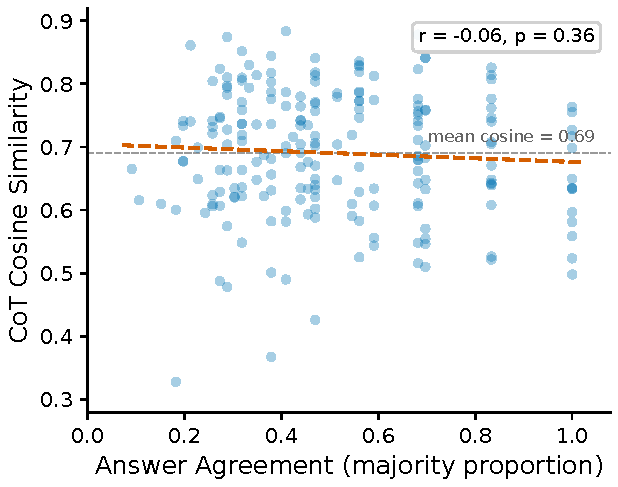
\includegraphics[width=0.85\columnwidth]{figures/fig3_process_kappa_scatter.pdf}
\caption{Answer agreement vs.\ CoT cosine similarity (Mistral-7B, FOLIO, $n{=}204$). Flat regression ($r = -0.06$, $p = 0.36$); stronger models show significant positive correlation ($r = +0.24$, Qwen-14B; Table~\ref{tab:cross-model-process}).}
\label{fig:process-kappa}
\end{figure}


\section{Extraction Error Taxonomy}
\label{app:extraction}
\label{sec:extraction-taxonomy}

Constraints must discriminate between candidate answers for MAX-SAT to produce a ranking different from majority vote. We measure discriminative power at two levels on Qwen2.5-14B across FOLIO and ProofWriter ($n = 804$). At the source-trace level, 39.2\% of total constraint weight originates from traces whose answer differs from the plurality, but only 12.1\% of individual constraints fall into this minority category. At the Z3 semantic level, 91.8\% of constraints [95\% CI: 91.2, 92.4] are technically discriminative, producing different satisfiability outcomes when evaluated against different candidate answers. Only 8.2\% are non-discriminative.

The high discriminative rate does not translate into accuracy gains because discrimination mirrors the model's own answer distribution. Each trace produces constraints with its own variable names, so Z3 treats identically-intended propositions as unrelated symbols; among cross-answer constraint pairs, 56.4\% share zero Z3 variables. This variable isolation means constraints from different traces are trivially jointly satisfiable, and MAX-SAT retains nearly all of them regardless of source answer. Removing the 8.2\% non-discriminative constraints yields zero accuracy improvement. The discriminative majority does not provide independent signal; it reinforces the majority answer that SC would already select. This confirmation bias, not a lack of discrimination, explains why SICA degenerates to majority voting (Appendix~\ref{app:ablation}).


\section{Hyperparameter Sensitivity}
\label{app:sensitivity}
\label{sec:k-sensitivity}
\label{sec:t-sensitivity}

\subsection{K Sensitivity}

Figure~\ref{fig:k-sensitivity} shows SICA $\Delta$ as a function of the number of sampled traces $K$ for Mistral-7B on FOLIO ($n = 204$, no fixed seed). The relationship is non-monotonic: $K = 4$ yields $\Delta = -1.47$\,pp, $K = 8$ yields $\Delta = -1.96$\,pp, $K = 12$ reaches $\Delta = +3.43$\,pp, $K = 16$ drops to $\Delta = +1.47$\,pp, and $K = 20$ partially recovers to $\Delta = +1.96$\,pp. The recovery at $K = 20$ rules out a simple peaked pattern, but $K = 12$ remains the only setting with $\Delta > 2$\,pp ($p = 0.092$, marginal).

The apparent $\Delta$ peak at $K = 12$ is confounded with SC baseline. SICA absolute accuracy plateaus at 59.31\% (121/204) for $K \geq 12$: identical at $K = 12$ and $K = 20$. The $\Delta$ variation across these settings is driven primarily by SC fluctuations rather than by SICA improvement. $K = 12$ produces a relatively low SC (55.88\%), placing it in the intermediate-SC region; $K = 8$ (SC $= 58.33\%$) and $K = 20$ (SC $= 57.35\%$) have higher baselines, compressing $\Delta$ even though SICA accuracy does not change for $K \geq 12$. Additional traces beyond $K = 12$ provide no benefit to SICA absolute performance, consistent with the constraint quality bottleneck. The $K = 12$ $\Delta$ captures only 25.0\% of the oracle ceiling ($+13.73$\,pp).

\begin{figure}[h]
\centering

\includegraphics[width=\columnwidth]{f3_k_sensitivity}
\caption{SICA $\Delta$ (pp) vs.\ number of traces $K$ for Mistral-7B on FOLIO ($n = 204$, default seed, $T = 0.7$). Non-monotonic pattern: SICA accuracy plateaus at 59.31\% for $K \geq 12$; the apparent $\Delta$ peak at $K = 12$ partly reflects a relatively low SC baseline (55.88\%) at that point. Error bars: 95\% bootstrap CI.}
\label{fig:k-sensitivity}
\end{figure}

\subsection{Temperature Sensitivity}

Temperature sensitivity on Mistral-7B FOLIO ($n = 204$, default seed) reveals a sharp isolated peak rather than a smooth trend. Across four temperature settings, only $T = 0.7$ produces a positive effect: $T = 0.3$ yields $\Delta = -1.47$\,pp (SC $= 58.33\%$), $T = 0.5$ yields $\Delta = -0.98$\,pp (SC $= 58.33\%$), $T = 0.7$ yields $\Delta = +3.43$\,pp (SC $= 55.88\%$), and $T = 1.0$ yields $\Delta = 0.00$\,pp (SC $= 55.39\%$). All other temperatures yield negative or null effects, and the single positive result at $T = 0.7$ is confounded with SC baseline. Combined with the seed sensitivity (0 of 4 seeds reaching $p < 0.05$ at $T = 0.7$), the positive trend depends on a specific combination of temperature, seed, and baseline accuracy that same-model sampling rarely achieves.

The parallel between $K$ and $T$ sensitivity points to a common underlying variable. In both sweeps, the setting that produces the largest SICA gain also produces a relatively low SC baseline (55.88\%), which places it in the intermediate-SC region. The hyperparameters themselves ($K$, $T$) are not the causal driver; they modulate SC level, and it is the SC level that determines whether SICA has operating room.


\section{Entropy Decomposition}
\label{app:entropy}
\label{sec:entropy}

We partition problems by trace agreement: high-entropy (majority count $\leq 8$ out of $K = 12$) and low-entropy (majority count $\geq 9$). Table~\ref{tab:entropy} reports SICA $\Delta$ within each partition across eight model-dataset conditions.

\begin{table}[h]
\centering
\small
\caption{Entropy decomposition of SICA $\Delta$ (pp). High-entropy: majority count $\leq 8$; low-entropy: majority count $\geq 9$. $^\dagger$Partial data (180/600). Pre-tiebreaking SC values; pattern robust to D064 correction.}
\label{tab:entropy}
\begin{tabular}{@{}llrrrr@{}}
\toprule
Model & Dataset & \multicolumn{2}{c}{High-entropy} & \multicolumn{2}{c}{Low-entropy} \\
\cmidrule(lr){3-4} \cmidrule(lr){5-6}
 & & $n$ & $\Delta$ & $n$ & $\Delta$ \\
\midrule
Mistral-7B & FOLIO & 78 & $\mathbf{+12.8}$ & 126 & 0.0 \\
Mistral-7B (s123) & FOLIO & 77 & $\mathbf{+9.1}$ & 127 & 0.0 \\
Mistral-7B (s456) & FOLIO & 75 & $-$1.3 & 129 & 0.0 \\
Mistral-7B & PW-D5 & 267 & $-$4.9 & 333 & $-$1.2 \\
Qwen2.5-14B & FOLIO & 37 & $-$8.2 & 167 & $-$0.6 \\
Qwen2.5-14B & LogiQA & 23 & $-$4.3 & 177 & 0.0 \\
Qwen2.5-7B & FOLIO & 47 & $-$2.1 & 157 & 0.0 \\
LLaMA-3.1-8B$^\dagger$ & PW-D5 & 76 & $-$3.9 & 104 & $-$1.9 \\
\bottomrule
\end{tabular}
\end{table}

Two patterns emerge. First, low-entropy problems produce $\Delta \approx 0$\,pp across all eight conditions: when traces agree, constraints carry no information beyond the majority vote.

Second, the direction of SICA's effect on high-entropy problems depends on the accuracy regime, not on entropy alone. In the intermediate-SC region (Mistral-7B on FOLIO, default-seed and seed-123 runs), high-entropy $\Delta$ reaches $+12.8$ and $+9.1$\,pp: traces genuinely disagree, and constraints from correct-answer traces provide discriminative signal that resolves the disagreement. In Type~A conditions (Qwen2.5-14B on FOLIO, $\Delta = -8.2$\,pp), high-entropy problems represent rare deviations from a strong model's consensus; constraints inherit the model's confirmation bias. In Type~C (Mistral-7B on ProofWriter, $\Delta = -4.9$\,pp), high-entropy problems reflect systematic errors. The mechanism is not entropy per se but the interaction of entropy with model capability.


\section{Failure Mode Analysis}
\label{app:failure-modes}
\label{sec:failure-modes}

The regime-dependent pattern in Table~\ref{tab:main_results} reflects three distinct failure modes of self-extracted logical constraints.

\paragraph{Type A: confirmation bias (SC $\geq$ $\sim$60\%).} Strong models produce consistent reasoning traces, and constraints extracted from those traces mirror the answer distribution. When most constraints support the same candidate, MAX-SAT excludes few clauses ($|\mathcal{C}^{\setminus}| \approx 0$), the penalty term in Eq.~\ref{eq:score} vanishes, and the scoring function degenerates to weighted vote counting (Eq.~\ref{eq:degenerate}). SICA and SC then produce identical predictions. The ablation in Appendix~\ref{app:ablation} confirms this empirically: on Qwen2.5-14B (FOLIO + ProofWriter, $n = 804$), MAX-SAT and count-only baselines agree on 803 of 804 predictions.

\paragraph{Type B: non-formalizable domains.} LogiQA problems require pragmatic and contextual reasoning that resists clean logical formalization. Qwen2.5-14B on LogiQA achieves an extraction rate of 86.4\%, but the resulting constraints have a contradiction rate of only 0.8\%: extracted formulas rarely conflict across traces, leaving MAX-SAT with no logical tension to exploit. Mistral-7B on LogiQA sits in the same SC range (50.00\%) yet produces $\Delta = +1.50$\,pp ($p = 0.581$); Qwen2.5-14B on the same domain yields $\Delta = -1.00$\,pp ($p = 0.625$). Neither model benefits, confirming that the right accuracy regime is necessary but not sufficient when the domain resists formalization.

\paragraph{Type C: error amplification (SC $\leq$ $\sim$40\%).} When model accuracy is low, the majority of traces reach incorrect answers. Constraints extracted from wrong traces encode incorrect reasoning as formal rules. Z3 treats these rules as soft clauses with weight proportional to their frequency, so the solver preferentially satisfies the wrong constraints and penalizes traces that happen to reach the correct answer. Mistral-7B on ProofWriter ($\Delta = -2.83$\,pp, raw $p = 0.014$; BH adj.\ $p = 0.042$) demonstrates this effect: SICA converts a weak positive signal in trace diversity into a net negative by formalizing the errors.


\section{Cross-Model Confirmation Bias}
\label{app:cross-model-bias}

Table~\ref{tab:cross-model-bias} reports MaxSAT-weighted confirmation bias metrics across three model families on FOLIO ($n = 204$). Weighted bias ratio and wrong-supporting constraint percentage both decrease with model capability, while SICA's accuracy effect shifts from positive (Mistral, intermediate-SC regime) to negative (LLaMA, high-SC regime). Raw bias ratios ($4.97\times$, $3.85\times$, $2.88\times$) are reported in \S\ref{sec:confirmation-bias}. LLaMA weighted BR CI: [2.19, 3.28].

\begin{table}[h]
\centering
\small
\caption{Cross-model confirmation bias on FOLIO ($n = 204$, $K = 12$). BR (wtd.): MaxSAT-weighted ratio of error-supporting constraints on incorrect vs.\ correct problems. Wrong \%: weighted fraction of constraints supporting the incorrect majority on error problems. $\Delta$: SICA $-$ SC (pp).}
\label{tab:cross-model-bias}
\begin{tabular}{@{}lrrr@{}}
\toprule
Model & BR (wtd.) & Wrong (\%) & $\Delta$ (pp) \\
\midrule
Mistral-7B & $4.24\times$ & 80.9 & $+$4.90 \\
Qwen2.5-14B & $3.69\times$ & 78.7 & $-$0.98 \\
LLaMA-3.1-8B & $2.66\times$ & 72.7 & $-$4.41 \\
\bottomrule
\end{tabular}
\end{table}

\paragraph{Frontier model universality.}
\label{app:frontier-scb}
Table~\ref{tab:frontier-scb} (main text, \S\ref{sec:confirmation-bias}) extends confirmation bias analysis to nine models spanning 7B open-source to frontier closed-source. All models exhibit $\text{BR} > 1$ (range: $1.66$--$4.97\times$). Extraction context varies: open-source models use self-extraction (the model extracts constraints from its own traces); frontier models use cross-model extraction (Mistral-7B extracts FOL from the target model's traces), as closed-source APIs do not expose internal representations suitable for direct symbolic extraction.

\paragraph{ProcessSim definition.}
\label{app:process-sim}
Process similarity is the mean pairwise cosine similarity of TF-IDF trace representations:
\begin{equation}
\label{eq:process-sim}
\text{ProcessSim}(q) = \frac{2}{K(K{-}1)} \sum_{i < j} \cos(\mathbf{v}_i^q, \mathbf{v}_j^q),
\end{equation}
where $\mathbf{v}_i^q$ is the TF-IDF vector of trace $t_i$ for question $q$.

\paragraph{Process-$\kappa$ gradient.}
\label{app:process-gradient}
Under cross-model extraction (Mistral-7B extracts FOL from other models' traces), SICA gain decreases monotonically with process-level cosine similarity (Table~\ref{tab:process-gradient}; Spearman $\rho = -1.0$, $n = 5$, one-tailed $p = 0.0083$). Gain requires two conditions: diverse traces (low $\kappa_{\text{proc}}$) \emph{and} substantial self-bias (high BR). R1-Distill-8B satisfies both ($\kappa_{\text{proc}} = 0.248$, $\text{BR} = 2.92$) and gains $+2.45$\,pp; o3 has moderate trace diversity ($\kappa_{\text{proc}} = 0.596$) but near-minimal bias ($\text{BR} = 1.66$, exhibiting a bimodal error pattern: 82\% of error problems have $\text{BR} = \infty$ but low finite-BR), yielding $\Delta = 0$.

\begin{table}[h]
\centering
\small
\caption{Process-$\kappa$ gradient under cross-model extraction (Mistral-7B $\rightarrow$ target model traces, FOLIO). $\kappa_{\text{proc}}$: process-level cosine similarity. $\Delta$: SICA $-$ SC (pp). Spearman $\rho(\kappa_{\text{proc}} \rightarrow \Delta) = -1.0$, $p = 0.0083$. $^*$Interim ($n = 95/204$).}
\label{tab:process-gradient}
\begin{tabular}{@{}lrrr@{}}
\toprule
Model & $\kappa_{\text{proc}}$ & $\Delta$ (pp) & BR \\
\midrule
R1-Distill-8B & 0.248 & $+$2.45 & 2.92 \\
gpt-5.5 & 0.563 & $+$0.49 & 3.48 \\
o3 & 0.596 & 0.00 & 1.66 \\
Gemini-2.5-Pro$^*$ & 0.790 & $-$1.05 & 2.79 \\
gpt-4.1 & 0.792 & $-$1.47 & 2.70 \\
\bottomrule
\end{tabular}
\end{table}


\section{Independence-Accuracy Scatter Plot}
\label{app:kappa-scatter}

\begin{figure}[h]
\centering
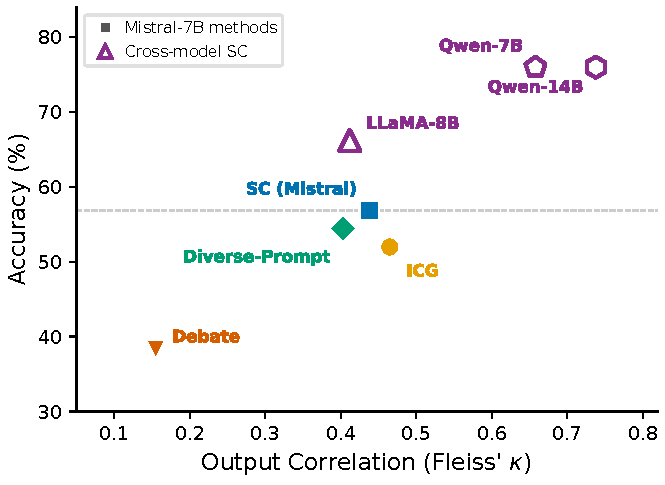
\includegraphics[width=\columnwidth]{figures/f6_kappa_accuracy_scatter}
\caption{Independence-accuracy trade-off across aggregation methods (Mistral-7B, filled markers) and model families (LLaMA-3.1-8B, Qwen2.5-7B, Qwen2.5-14B; open markers) on FOLIO ($n = 204$). Same-model methods cluster at $\kappa \approx 0.40$--$0.47$ (gray band), while cross-model SC shows stronger correlations ($\kappa = 0.41$--$0.74$) at higher accuracy. Debate breaks correlation ($\kappa = 0.15$) at catastrophic accuracy cost. Dashed line: Mistral-7B SC baseline.}
\label{fig:kappa-accuracy}
\end{figure}

\begin{table}[h]
\centering
\small
\caption{Independence-accuracy trade-off (FOLIO, $n = 204$). Top: aggregation methods on Mistral-7B; bottom: SC across three model families. All families produce $\kappa \geq 0.41$, confirming an architecture-independent ceiling. $\kappa$: Fleiss' kappa on raw answers.}
\label{tab:kappa_generalization}
\setlength{\tabcolsep}{3.5pt}
\begin{tabular}{@{}llccrr@{}}
\toprule
Model & Aggregation & $\kappa$ & Eff-$K$ & $K$ & Acc.\ (\%) \\
\midrule
Mistral-7B & Debate & 0.15 & 4.44 & 12 & 38.24 \\
& Diverse-Prompt & 0.40 & 2.21 & 12 & 54.41 \\
& Self-Consistency & 0.44 & 2.02 & 10 & 56.86 \\
& ICG & 0.47 & 1.93 & 10 & 51.96 \\
\addlinespace
LLaMA-3.1-8B & Self-Consistency & 0.41 & 2.17 & 12 & 66.18 \\
Qwen2.5-7B & Self-Consistency & 0.66 & 1.46 & 12 & 75.98 \\
Qwen2.5-14B & Self-Consistency & 0.74 & 1.32 & 12 & 75.98 \\
\bottomrule
\end{tabular}
\end{table}

\paragraph{Trace independence metrics.}
\label{app:trace-independence}

Table~\ref{tab:independence} reports the full 15-condition breakdown of Fleiss' $\kappa$ and Effective-K at $K = 12$, referenced in \S\ref{sec:effective-k}.

\begin{table}[h]
\centering
\small
\setlength{\tabcolsep}{3pt}
\caption{Trace independence metrics ($K = 12$, sorted by $\kappa$ descending). $\kappa$: Fleiss' Kappa. $K_{\text{eff}}$: Effective-K (Eq.~\ref{eq:effk}). SC: Self-Consistency baseline. $\Delta$: SICA $-$ SC (pp). {*}\,$p < 0.05$ (uncorrected; BH adj.\ $p = 0.042$, $m{=}6$); positive $\Delta$ values do not reach significance. multi-T $= T \in \{0.3, 0.7, 1.2\}$, 4 traces each. $^{\dag}$\,$\kappa$ computed in an earlier pipeline run; all other rows recomputed from per-problem vote distributions with answer labels normalized to canonical categories.}
\label{tab:independence}
\begin{tabular}{@{}llccrr@{}}
\toprule
Model & Condition & $\kappa$ & $K_{\text{eff}}$ & SC (\%) & $\Delta$ (pp) \\
\midrule
Qwen3 (think) & FOLIO & 0.91$^{\dag}$ & 1.09 & 86.27 & $+$0.49 \\
Qwen2.5-14B & LogiQA & 0.82 & 1.20 & 79.00 & $-$1.00 \\
Qwen3 & FOLIO & 0.79 & 1.24 & 83.33 & $+$1.47 \\
Qwen2.5-14B & FOLIO & 0.74 & 1.31 & 75.98 & $-$0.49 \\
Qwen2.5-7B & FOLIO & 0.66$^{\dag}$ & 1.46 & 75.98 & $+$0.49 \\
\addlinespace
Mistral-7B ($T{=}0.3$) & FOLIO & 0.53$^{\dag}$ & 1.77 & 58.33 & $-$1.47 \\
Mistral-7B ($T{=}0.5$) & FOLIO & 0.52$^{\dag}$ & 1.80 & 58.33 & $-$0.98 \\
Mistral-7B & LogiQA & 0.51 & 1.81 & 50.00 & $+$1.50 \\
Mistral-7B ($T{=}1.0$) & FOLIO & 0.48$^{\dag}$ & 1.91 & 55.39 & 0.00 \\
Mistral-7B & FOLIO & 0.46 & 1.98 & 55.88 & $+$3.43 \\
Mistral-7B (s123) & FOLIO & 0.46 & 1.99 & 54.41 & $+$2.94 \\
Mistral-7B (s456) & FOLIO & 0.46 & 1.99 & 55.88 & 0.00 \\
Mistral-7B (s789) & FOLIO & 0.45 & 2.03 & 59.31 & $-$2.45 \\
Mistral-7B (multi-T) & FOLIO & 0.43 & 2.11 & 57.84 & 0.00 \\
Mistral-7B & PW-D5 & 0.19 & 3.94 & 39.33 & $\mathbf{-2.83}${*} \\
\bottomrule
\end{tabular}
\end{table}

\section{Cross-Model Kappa Analysis}
\label{app:cross-model-kappa}

Table~\ref{tab:cross_model_kappa} compares trace independence across three model families on the same benchmarks. On FOLIO ($n = 204$), all four models produce $\kappa \geq 0.41$: LLaMA-3.1-8B ($\kappa = 0.41$), Mistral-7B ($\kappa = 0.46$), Qwen2.5-7B ($\kappa = 0.66$), and Qwen2.5-14B ($\kappa = 0.74$). The bottleneck is architecture-independent---no family escapes the correlation floor. Within the Qwen family, $\kappa$ increases from 0.66 (7B) to 0.74 (14B), but Mistral-7B (7B) and LLaMA-3.1-8B (8B) differ by $\Delta\kappa = 0.05$ despite belonging to different families, suggesting that cross-family variation ($\Delta\kappa$ up to 0.20 at similar scale) exceeds within-family scale effects ($\Delta\kappa = 0.08$). Disentangling scale from architecture requires controlled same-family experiments across $\geq$3 scales.

\begin{table}[h]
\centering
\small
\caption{Cross-model trace independence ($K = 12$, SC aggregation, FOLIO + ProofWriter). Higher $\kappa$ indicates stronger correlation and lower effective sample size.}
\label{tab:cross_model_kappa}
\begin{tabular}{@{}llccr@{}}
\toprule
Model & Dataset & $\kappa$ & $K_{\text{eff}}$ & SC (\%) \\
\midrule
Qwen2.5-14B & FOLIO & 0.74 & 1.32 & 75.98 \\
Qwen2.5-7B & FOLIO & 0.66 & 1.46 & 75.98 \\
Mistral-7B & FOLIO & 0.46 & 1.98 & 55.88 \\
LLaMA-3.1-8B & FOLIO & 0.41 & 2.17 & 66.18 \\
\addlinespace
Qwen2.5-14B & PW-D5 & 0.62 & 1.54 & --- \\
Mistral-7B & PW-D5 & 0.19 & 3.94 & 39.33 \\
\bottomrule
\end{tabular}
\end{table}


\section{Cross-Model Process-Level Independence}
\label{app:cross-model-process}

Table~\ref{tab:cross-model-process} extends the process-level independence analysis (\S\ref{sec:process-kappa}) to four model families on FOLIO ($n = 204$). Mean pairwise cosine similarity of TF-IDF trace representations exceeds answer-level $\kappa$ in every family, but the gap is model-strength dependent: it narrows from $0.31$ (LLaMA) and $0.23$ (Mistral) to $0.02$ (Qwen-14B). For weaker models ($r \approx 0$), answer diversity does not reflect reasoning diversity---process-convergent but answer-divergent trace pairs constitute 9.5\% of all pairs on Mistral-7B versus 2.5--3.2\% on other families. For stronger models ($r \approx 0.23$, $p \leq 0.001$), process and answer agreement align, and answer-level $\kappa$ already captures the bottleneck. Process-$\kappa$ thus provides a crucial additional diagnostic specifically for weaker models, where answer-level metrics underestimate reasoning homogeneity.

\begin{table}[h]
\centering
\small
\caption{Cross-model process-level independence on FOLIO ($n = 204$, $K = 12$). Mean Cosine: mean pairwise TF-IDF cosine similarity of reasoning traces (Eq.~\ref{eq:process-sim}). Answer $\kappa$: per-question answer agreement. Gap: Cosine $-$ $\kappa$. $r$: Pearson correlation between ProcessSim and answer agreement. Conv.: fraction of process-convergent but answer-divergent trace pairs. {*}{*}\,$p < 0.01$; {*}{*}{*}\,$p < 0.001$.}
\label{tab:cross-model-process}
\resizebox{\columnwidth}{!}{%
\begin{tabular}{@{}lcccrlr@{}}
\toprule
Model & Mean Cos. & Ans.\ $\kappa$ & Gap & $r$ & $p$ & Conv.\ (\%) \\
\midrule
Mistral-7B & 0.690 & 0.460 & 0.230 & $-$0.064 & 0.362 & 9.5 \\
LLaMA-3.1-8B & 0.759 & 0.447 & 0.312 & $-$0.001 & 0.985 & 3.2 \\
Qwen2.5-7B & 0.790 & 0.658 & 0.132 & $+$0.226 & 0.001{*}{*} & 2.8 \\
Qwen2.5-14B & 0.766 & 0.744 & 0.022 & $+$0.244 & ${<}$0.001{*}{*}{*} & 2.5 \\
\bottomrule
\end{tabular}}
\end{table}

\paragraph{Representation robustness.} Replacing TF-IDF with SBERT embeddings (all-MiniLM-L6-v2) yields ProcessSim $= 0.91$ (vs.\ TF-IDF $0.74$), widening the gap over answer-level $\kappa = 0.55$. The process homogeneity finding is robust to representation choice.

\section{Constraint Quality Across Methods}
\label{app:constraint-quality}

Table~\ref{tab:constraint_quality} compares constraint quality metrics across the three method-level interventions on Mistral-7B FOLIO ($n = 204$). Standard SICA extracts from reasoning traces and achieves the highest parse rate (97.1\%) but also the highest redundancy (42.9\%): nearly half of all constraints are syntactic duplicates across the 12 traces, quantifying the co-sourcing effect of same-model generation. ICG generates constraints directly from the problem statement without trace conditioning. Its lower parse rate (74.6\%) reflects the difficulty of standalone formalization at the 7B scale, though successfully parsed constraints compile at a higher rate (99.4\% vs.\ 96.5\%). ICG produces fewer unique constraints per question (24.9 vs.\ 39.3) with lower redundancy (32.3\%), consistent with the absence of trace-level repetition. Contrastive scoring generates pro and con constraint sets for each candidate answer. The format yields far fewer unique constraints per question (9.2) with zero redundancy (each pro/con pair is structurally distinct), but 62.7\% of constraints are trivially satisfied by Z3---they impose no logical tension and cannot discriminate between candidates. Only 51.0\% of Contrastive constraints are discriminative, compared to 81.4\% for standard SICA and 77.0\% for ICG.

\begin{table}[h]
\centering
\small
\caption{Constraint quality metrics across method-level interventions (Mistral-7B, FOLIO, $n = 204$). Parse: fraction of extraction attempts yielding valid JSON. Z3 Compile: fraction compiling to Z3 formulas. Unique/q: mean unique constraints per question. Redundancy: fraction of constraints duplicated across traces. Disc.: fraction discriminative (different Z3 outcome per candidate). Triv.\ Sat.: fraction trivially satisfied (no logical tension).}
\label{tab:constraint_quality}
\resizebox{\columnwidth}{!}{%
\begin{tabular}{@{}l rrrrrr@{}}
\toprule
Method & Parse & Z3 & Uniq/q & Redund. & Disc. & Triv.\ Sat. \\
\midrule
Standard SICA & 97.1\% & 96.5\% & 39.3 & 42.9\% & 81.4\% & --- \\
ICG & 74.6\% & 99.4\% & 24.9 & 32.3\% & 77.0\% & --- \\
Contrastive & 74.0\% & 94.4\% & 9.2 & 0.0\% & 51.0\% & 62.7\% \\
\bottomrule
\end{tabular}}
\end{table}

\paragraph{Per-trace constraint yield uniformity.}
\label{app:yield-cv}

Observation~1 assumes approximately uniform constraint yield per trace within each answer group. We verify this on Mistral-7B FOLIO ($K{=}12$, $n{=}204$). Per-problem yield CV (coefficient of variation across traces within each problem) has median $0.257$ and mean $0.319$; 64.2\% of problems fall below $\text{CV} = 0.3$, and 91.2\% below $0.5$, supporting the uniformity assumption. Majority-answer traces average $5.61$ constraints and minority-answer traces $6.04$ (Mann--Whitney $p = 5.2 \times 10^{-6}$); correct-answer traces average $5.41$ and incorrect $6.05$ ($p = 5.3 \times 10^{-11}$). Although statistically significant, the absolute difference (${\sim}0.6$ constraints, $< 12\%$) is insufficient to alter the argmax-preservation result: SICA and SC select the same answer on ${>}96\%$ of problems regardless of yield variation.

\section{Error Categorization of Method-Level Interventions}
\label{app:error-categorization}

We categorize discordant predictions (where the method and SC disagree) for Debate and Contrastive on FOLIO ($n = 204$) to understand why these interventions degrade accuracy.

\paragraph{Debate discordant analysis.} Debate produces 60 correct$\to$wrong flips and 22 wrong$\to$correct flips on FOLIO. Answer-type breakdown reveals that False-labeled questions are most vulnerable: 82.8\% of False questions that SC answers correctly are flipped by Debate, compared to 63.9\% for True and 25.5\% for Unknown. Counterintuitively, failures concentrate not where debate breaks down but where it succeeds most thoroughly: discordant questions average 2.93 effective debate rounds (proposer-critic exchanges producing substantive updates) versus 2.52 for concordant ones. More extensive same-model debate produces more confident but incorrect constraints, consistent with the independence limitation---the critic draws on the same model distribution as the proposer, reinforcing shared biases rather than correcting them.

\paragraph{Contrastive discordant analysis.} Contrastive produces 34 discordant questions on FOLIO. All 34 produced non-degenerate scores (both pro and con constraint sets non-empty), compared to 20.1\% degenerate scores in the full sample. This indicates that scoring failures on discordant questions stem from systematic pro-bias rather than missing constraints. Among discordant questions, 97.1\% contain negation words in the problem statement versus 76.5\% in the full sample, suggesting that negation-bearing problems are particularly susceptible to pro-constraint imbalance. The average pro/con score ratio is 1.0 for discordant questions versus 0.68 for the full sample: the method generates balanced-looking scores that mask directional errors.

\paragraph{Cross-method overlap.} Of the 79 unique questions on which either method disagrees with SC, only 15 overlap between Debate and Contrastive (Jaccard index $= 0.19$). All 15 shared discordant questions contain negation words. The low overlap confirms that the two methods attack different vulnerability types---Debate through extended same-model argumentation that amplifies confident errors, Contrastive through pro-bias in constraint generation---while sharing a common root cause in correlated same-model voting: both methods rely on the same model's output distribution and cannot introduce genuinely independent signal.


\section{TOST Equivalence Tests}
\label{app:tost}

We apply two one-sided tests (TOST) \citep{lakens2017equivalence} with equivalence margin $\pm 2$\,pp to all 16 non-degenerate SICA--SC comparisons, classifying each condition as \emph{equivalent} (TOST significant), \emph{genuinely different} (McNemar $p < 0.05$ and TOST not significant), or \emph{underpowered} (neither test significant). Four conditions are equivalent, confirming that SICA and SC produce statistically indistinguishable accuracy. Two conditions show genuine differences, both negative: Mistral-7B ProofWriter ($-2.83$\,pp, $p = 0.014$) and Qwen2.5-14B ProofWriter ($-2.50$\,pp, $p = 0.011$). The remaining ten conditions are underpowered, reflecting the limited statistical power at $n{=}200$--$204$ for detecting $|\Delta| \leq 2$\,pp effects.

\paragraph{Margin sensitivity.} Table~\ref{tab:tost-sensitivity} shows that the classification is robust across margins: regardless of the chosen margin, no condition shows a significant positive SICA effect.

\begin{table}[h]
\centering
\small
\caption{TOST classification sensitivity across equivalence margins (16 non-degenerate conditions).}
\label{tab:tost-sensitivity}
\begin{tabular}{@{}lccc@{}}
\toprule
Margin & Equivalent & Different & Underpowered \\
\midrule
$\pm 1$\,pp & 0 & 2 & 14 \\
$\pm 2$\,pp & 4 & 2 & 10 \\
$\pm 3$\,pp & 10 & 0 & 6 \\
\bottomrule
\end{tabular}
\end{table}

\paragraph{Relative-margin TOST.}
\label{app:relative_tost}
The absolute $\pm 2$\,pp margin is more stringent at high baselines ($\pm 2.4\%$ relative at SC $= 85\%$) than low ones ($\pm 5.1\%$ at SC $= 39\%$). A relative $\pm 5\%$ of SC margin addresses this asymmetry: 8 conditions are equivalent, 2 genuinely different (both negative), and 6 underpowered. The additional four equivalent conditions are all high-SC ($\geq 75\%$), where the wider relative band captures practical indistinguishability. No condition shows a significant positive effect under either margin.

\paragraph{Conditional Correction Ratio data.}
\label{app:cil-data}

\begin{table}[h]
\centering
\small
\setlength{\tabcolsep}{3pt}
\caption{Conditional Correction Ratio across eight verifier--generator conditions. $\text{CCR} > 0$: cross-arch NLI on ProofWriter. $\text{CCR} < 0$: same-model SICA or weak capability gap.}
\label{tab:cil_main}
\begin{tabular}{@{}llrr@{}}
\toprule
Generator--Verifier & Dataset & CCR & $\Delta$ (pp) \\
\midrule
Mistral $\times$ BART-NLI & PW & $+$1.86 & $+$5.17 \\
Mistral $\times$ DeBERTa-NLI & PW & $+$1.67 & $+$6.67 \\
Mistral $\times$ RoBERTa-NLI & PW & $+$1.42 & $+$4.17 \\
\addlinespace
Qwen-14B $\times$ DeBERTa-NLI & PW & $-$0.21 & $+$0.33 \\
Mistral $\times$ DeBERTa-NLI & FOLIO & $-$0.47 & $+$2.94 \\
\addlinespace
Mistral $\times$ SICA & FOLIO & $-$2.93 & $+$3.43 \\
Qwen-14B $\times$ SICA & PW & $-$4.21 & $-$2.50 \\
Mistral $\times$ SICA & PW & $-$4.61 & $-$2.83 \\
\bottomrule
\end{tabular}
\end{table}

\paragraph{Disagreement-Routed Cascade details.}
\label{app:drc}
DRC invokes NLI only when SC consensus falls below threshold $\tau$, avoiding unnecessary verifier calls on high-agreement problems. Gains concentrate on weak generators (SC $< 40\%$), consistent with the capability-gap hypothesis (\S\ref{sec:cross-arch}). Regime-dependent bottleneck analysis appears in Appendix~\ref{app:2x2}.

\begin{table}[h]
\centering
\small
\caption{DRC on Mistral-7B ($K{=}12$, DeBERTa-large-mnli, $w{=}3$). $\tau{=}0.7$ recovers 83--90\% of full-combo gain at ${\sim}35\%$ NLI cost across both datasets.}
\label{tab:drc}
\setlength{\tabcolsep}{3pt}
\begin{tabular}{@{}llcccc@{}}
\toprule
Dataset & Method & Acc.\ & NLI Calls & Cost & Recovery \\
\midrule
\multirow{3}{*}{PW-D5} & SC only & 39.33\% & 0/600 & 0\% & --- \\
& \textbf{DRC $\tau{=}0.7$} & \textbf{45.33\%} & \textbf{207/600} & \textbf{34.5\%} & \textbf{90.0\%} \\
& Full combo & 46.00\% & 600/600 & 100\% & 100\% \\
\midrule
\multirow{3}{*}{FOLIO} & SC only & 55.88\% & 0/204 & 0\% & --- \\
& \textbf{DRC $\tau{=}0.7$} & \textbf{58.33\%} & \textbf{71/204} & \textbf{34.8\%} & \textbf{83.3\%} \\
& Full combo & 58.82\% & 204/204 & 100\% & 100\% \\
\bottomrule
\end{tabular}
\end{table}

\section{Multi-Verifier NLI Results}
\label{app:multi-nli}

\begin{table}[h]
\centering
\small
\caption{Cross-architecture NLI combo on ProofWriter depth-5 ($n{=}600$, Mistral-7B traces, SC $= 39.33\%$). Three NLI verifiers $\times$ three weight settings. {*}\,$p < 0.05$;\enspace{**}\,$p < 0.01$;\enspace{***}\,$p < 0.001$ (McNemar).}
\label{tab:multi-nli}
\begin{tabular}{@{}llrrl@{}}
\toprule
Verifier & Standalone & $w$ & $\Delta$ (pp) & $p$ \\
\midrule
DeBERTa-MNLI & 55.00\% & 1 & $+$0.83 & n.s. \\
 & & 3 & $+$6.67 & ${<}0.001${***} \\
 & & 5 & $+$11.00 & ${<}0.001${***} \\
\addlinespace
RoBERTa-MNLI & 37.67\% & 1 & $-$0.17 & n.s. \\
 & & 3 & $+$4.17 & 0.003{**} \\
 & & 5 & $+$4.33 & 0.037{*} \\
\addlinespace
BART-MNLI & 46.17\% & 1 & 0.00 & n.s. \\
 & & 3 & $+$5.17 & ${<}0.001${***} \\
 & & 5 & $+$6.33 & 0.003{**} \\
\bottomrule
\end{tabular}\\[2pt]
{\footnotesize All verifiers fine-tuned on MultiNLI. Unknown recall ${<}3.5\%$ across all verifiers.}
\end{table}

\paragraph{Three-verifier BH correction.}
\label{app:3verifier-bh}
Table~\ref{tab:3verifier-bh} applies Benjamini--Hochberg correction across all 15 Mistral-7B verifier--weight conditions ($m{=}15$, $\alpha{=}0.05$; distinct from the $m{=}12$ cross-generator analysis in \S\ref{sec:cross-arch}). Ten of 15 conditions remain significant after correction, confirming that multi-verifier NLI gains are robust to multiple testing.

\begin{table}[h]
\centering
\small
\caption{BH correction across 3 verifiers $\times$ 5 weights on Mistral-7B ProofWriter ($n{=}600$, $m{=}15$). \checkmark: $p_{\text{BH}} < 0.05$.}
\label{tab:3verifier-bh}
\setlength{\tabcolsep}{4pt}
\begin{tabular}{@{}lcccccc@{}}
\toprule
Verifier & $w{=}1$ & $w{=}2$ & $w{=}3$ & $w{=}4$ & $w{=}5$ \\
\midrule
DeBERTa-MNLI & & \checkmark & \checkmark & \checkmark & \checkmark \\
RoBERTa-MNLI & & & \checkmark & \checkmark & \checkmark \\
BART-MNLI & & & \checkmark & \checkmark & \checkmark \\
\bottomrule
\end{tabular}\\[2pt]
{\footnotesize 10/15 significant at $\alpha{=}0.05$ after BH correction. All $w{=}1$ conditions and RoBERTa $w{=}2$ are non-significant.}
\end{table}

\section{Capability Gap Data Points}
\label{app:capability-gap}

\begin{figure}[t]
\centering
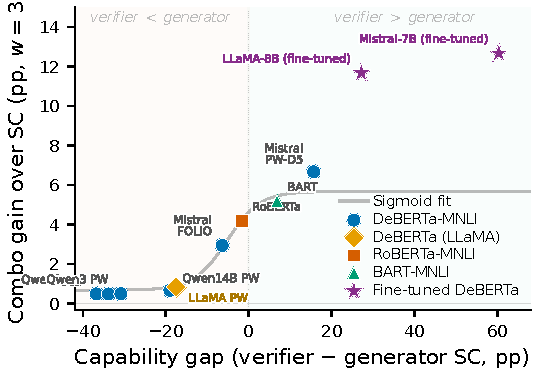
\includegraphics[width=0.78\columnwidth]{figures/capability_gap_scatter}
\caption{Combo gain vs.\ capability gap (verifier standalone $-$ generator SC) at $w{=}3$ across three NLI architectures. Gain decreases monotonically (Spearman $\rho = 1.0$, exact permutation $p = 0.003$, $n{=}6$; four of six conditions share the DeBERTa verifier---see Limitations); significant gains occur only for generators below the verifier's standalone accuracy. Stars: domain-adapted DeBERTa (99.67\% standalone, Table~\ref{tab:finetuned-nli}).}
\label{fig:capability-gap}
\end{figure}

Table~\ref{tab:cross_generator_nli} reports the controlled cross-generator comparison with DeBERTa-large-mnli on ProofWriter ($n{=}600$). We extend this analysis by pairing Mistral-7B with two additional NLI architectures: BART-large-mnli (46.17\% standalone, combo $+5.17$\,pp, $p = 0.0002$) and RoBERTa-large-mnli (37.67\% standalone, combo $+4.17$\,pp, $p = 0.003$). All three NLI architectures produce significant gains on Mistral-7B at $w \geq 3$.

Across all six ProofWriter verifier-generator pairs at $w{=}3$ (three verifiers $\times$ Mistral-7B plus three negative-gap generators $\times$ DeBERTa), combo gain decreases monotonically with the capability gap (Spearman $\rho = 1.0$, exact permutation $p = 0.003$, $n = 6$; however, four of six conditions share the DeBERTa verifier, which may reduce effective degrees of freedom---see Limitations; Figure~\ref{fig:capability-gap}). Significant $w{=}3$ gains are observed only for Mistral-7B (SC 39.33\%, below the verifier); the three above-verifier generators show no significant improvement at any $w$. After BH correction ($m{=}12$), two of twelve conditions survive: Mistral-7B $w{=}3$ (adj.\ $p = 6.78 \times 10^{-5}$) and $w{=}5$ (adj.\ $p = 7.41 \times 10^{-6}$).

\paragraph{Robustness check.} Including all nine conditions (three verifiers $\times$ three weight levels on Mistral-7B) yields Spearman $\rho = 0.836$ (exact permutation $p = 0.007$, $n = 9$), confirming that the monotonic trend is robust to the choice of weight parameter.

\paragraph{Full NLI combo with BH correction.}
\label{app:nli-combo-full}

\begin{table}[h]
\centering
\small
\caption{Full cross-generator NLI combo results on ProofWriter depth-5 ($n{=}600$) with Benjamini--Hochberg correction ($m{=}12$, $\alpha{=}0.05$). All conditions use DeBERTa-large-mnli verifier (55.00\% standalone). Two of twelve conditions survive correction (Mistral-7B $w{=}3$ and $w{=}5$). {***}\,$p_{\text{BH}} < 0.001$.}
\label{tab:nli-combo-full}
\setlength{\tabcolsep}{3.5pt}
\resizebox{\columnwidth}{!}{%
\begin{tabular}{@{}llrrrrl@{}}
\toprule
Generator & $w$ & Combo (\%) & $\Delta$ (pp) & $p_{\text{raw}}$ & $p_{\text{BH}}$ & \\
\midrule
\multirow{3}{*}{\shortstack[l]{Mistral-7B\\{\scriptsize SC\,39.33\%, gap\,$+$15.67}}}
  & 1 & 40.17 & $+$0.83 & .359 & .721 & \\
  & 3 & 46.00 & $+$6.67 & $1.13{\times}10^{-5}$ & $6.78{\times}10^{-5}$ & {***} \\
  & 5 & 50.33 & $+$11.00 & $6.18{\times}10^{-7}$ & $7.41{\times}10^{-6}$ & {***} \\
\addlinespace
\multirow{3}{*}{\shortstack[l]{LLaMA-3.1-8B\\{\scriptsize SC\,72.50\%, gap\,$-$17.50}}}
  & 1 & 73.33 & $+$0.83 & .359 & .721 & \\
  & 3 & 73.33 & $+$0.83 & .665 & .886 & \\
  & 5 & 72.00 & $-$0.50 & .871 & 1.000 & \\
\addlinespace
\multirow{3}{*}{\shortstack[l]{Qwen2.5-14B\\{\scriptsize SC\,74.00\%, gap\,$-$19.00}}}
  & 1 & 74.17 & $+$0.17 & 1.000 & 1.000 & \\
  & 3 & 74.67 & $+$0.67 & .503 & .755 & \\
  & 5 & 75.17 & $+$1.17 & .360 & .721 & \\
\addlinespace
\multirow{3}{*}{\shortstack[l]{Qwen3-14B\\{\scriptsize SC\,85.83\%, gap\,$-$30.83}}}
  & 1 & 86.00 & $+$0.17 & 1.000 & 1.000 & \\
  & 3 & 86.33 & $+$0.50 & .453 & .755 & \\
  & 5 & 87.00 & $+$1.17 & .210 & .721 & \\
\bottomrule
\end{tabular}}
\end{table}

\paragraph{BART-large-mnli cross-generator results.}

\begin{table}[h]
\centering
\small
\caption{Cross-generator NLI combo with BART-large-mnli verifier (46.17\% standalone) on ProofWriter depth-5 ($n{=}600$, $w{=}3$). Only Mistral-7B (below the verifier) gains significantly after BH correction.}
\label{tab:bart-combo-full}
\begin{tabular}{@{}lccrl@{}}
\toprule
Generator & SC (\%) & Combo (\%) & $\Delta$ (pp) & $p_{\text{BH}}$ \\
\midrule
Mistral-7B {\scriptsize (gap $+$6.84)} & 39.33 & 44.50 & $+$5.17 & .003{*} \\
LLaMA-3.1-8B {\scriptsize (gap $-$26.33)} & 72.50 & 72.50 & $\pm$0.00 & --- \\
Qwen2.5-14B {\scriptsize (gap $-$27.83)} & 74.00 & 75.50 & $+$1.50 & n.s. \\
Qwen3-14B {\scriptsize (gap $-$39.66)} & 85.83 & 86.50 & $+$0.67 & n.s. \\
\bottomrule
\end{tabular}
\end{table}

\paragraph{RoBERTa-large-mnli cross-generator results.}

\begin{table}[h]
\centering
\small
\caption{Cross-generator NLI combo with RoBERTa-large-mnli verifier (37.67\% standalone) on ProofWriter depth-5 ($n{=}600$, $w{=}3$). Only Mistral-7B (marginally above the verifier) gains significantly after BH correction.}
\label{tab:roberta-combo-full}
\begin{tabular}{@{}lccrl@{}}
\toprule
Generator & SC (\%) & Combo (\%) & $\Delta$ (pp) & $p_{\text{BH}}$ \\
\midrule
Mistral-7B {\scriptsize (gap $-$1.66)} & 39.33 & 43.50 & $+$4.17 & .016{*} \\
LLaMA-3.1-8B {\scriptsize (gap $-$34.83)} & 72.50 & 71.33 & $-$1.17 & n.s. \\
Qwen2.5-14B {\scriptsize (gap $-$36.33)} & 74.00 & 74.17 & $+$0.17 & n.s. \\
Qwen3-14B {\scriptsize (gap $-$48.16)} & 85.83 & 86.50 & $+$0.67 & n.s. \\
\bottomrule
\end{tabular}
\end{table}

\paragraph{FOLIO NLI combo results.}
\label{app:folio-nli-combo}

\begin{table}[h]
\centering
\small
\caption{NLI combo on FOLIO ($n{=}204$) with DeBERTa-large-mnli verifier (49.51\% standalone). No condition reaches significance; all generators exceed the verifier's standalone accuracy, consistent with the capability-gap pattern. SC baselines match the cross-model ablation traces (Table~\ref{tab:cross-model-ablation}).}
\label{tab:folio-nli-deberta}
\begin{tabular}{@{}lcccrl@{}}
\toprule
Generator & $w$ & SC (\%) & Combo (\%) & $\Delta$ (pp) & $p$ \\
\midrule
\multirow{3}{*}{Mistral-7B} & 1 & \multirow{3}{*}{55.88} & 56.37 & $+$0.49 & n.s. \\
 & 3 & & 58.82 & $+$2.94 & n.s. \\
 & 5 & & 59.80 & $+$3.92 & n.s. \\
\addlinespace
\multirow{3}{*}{LLaMA-3.1-8B} & 1 & \multirow{3}{*}{66.18} & 65.69 & $-$0.49 & n.s. \\
 & 3 & & 65.20 & $-$0.98 & n.s. \\
 & 5 & & 64.22 & $-$1.96 & n.s. \\
\addlinespace
\multirow{3}{*}{Qwen2.5-14B} & 1 & \multirow{3}{*}{75.98} & 76.96 & $+$0.98 & n.s. \\
 & 3 & & 75.49 & $-$0.49 & n.s. \\
 & 5 & & 73.53 & $-$2.45 & n.s. \\
\addlinespace
\multirow{3}{*}{Qwen3-14B} & 1 & \multirow{3}{*}{83.33} & 83.33 & $\pm$0.00 & n.s. \\
 & 3 & & 84.80 & $+$1.47 & n.s. \\
 & 5 & & 83.33 & $\pm$0.00 & n.s. \\
\bottomrule
\end{tabular}
\end{table}

\begin{table}[h]
\centering
\small
\caption{NLI combo on FOLIO ($n{=}204$) with BART-large-mnli verifier (47.06\% standalone). No positive improvement reaches significance; for Qwen2.5-14B the weak verifier produces a significant \emph{degradation} at $w{=}5$ ($p{=}.039$), consistent with the capability-gap pattern.}
\label{tab:folio-nli-bart}
\begin{tabular}{@{}lcccrl@{}}
\toprule
Generator & $w$ & SC (\%) & Combo (\%) & $\Delta$ (pp) & $p$ \\
\midrule
\multirow{3}{*}{Mistral-7B} & 1 & \multirow{3}{*}{55.88} & 54.90 & $-$0.98 & n.s. \\
 & 3 & & 56.37 & $+$0.49 & n.s. \\
 & 5 & & 56.86 & $+$0.98 & n.s. \\
\addlinespace
\multirow{3}{*}{LLaMA-3.1-8B} & 1 & \multirow{3}{*}{66.18} & 67.65 & $+$1.47 & n.s. \\
 & 3 & & 67.65 & $+$1.47 & n.s. \\
 & 5 & & 64.71 & $-$1.47 & n.s. \\
\addlinespace
\multirow{3}{*}{Qwen2.5-14B} & 1 & \multirow{3}{*}{75.98} & 76.47 & $+$0.49 & n.s. \\
 & 3 & & 75.00 & $-$0.98 & n.s. \\
 & 5 & & 72.55 & $-$3.43 & .039{*} \\
\addlinespace
\multirow{3}{*}{Qwen3-14B} & 1 & \multirow{3}{*}{83.33} & 83.33 & $\pm$0.00 & n.s. \\
 & 3 & & 84.31 & $+$0.98 & n.s. \\
 & 5 & & 82.84 & $-$0.49 & n.s. \\
\bottomrule
\end{tabular}
\end{table}

\begin{table}[h]
\centering
\small
\caption{NLI combo on FOLIO ($n{=}204$) with RoBERTa-large-mnli verifier (46.57\% standalone). Cross-verifier consistency: no positive gain reaches significance, and Qwen2.5-14B shows a significant \emph{degradation} at $w{=}5$ ($p{=}.012$)---the same capability-gap signature as BART.}
\label{tab:folio-nli-roberta}
\begin{tabular}{@{}lcccrl@{}}
\toprule
Generator & $w$ & SC (\%) & Combo (\%) & $\Delta$ (pp) & $p$ \\
\midrule
\multirow{3}{*}{Mistral-7B} & 1 & \multirow{3}{*}{55.88} & 56.37 & $+$0.49 & n.s. \\
 & 3 & & 57.84 & $+$1.96 & n.s. \\
 & 5 & & 58.82 & $+$2.94 & n.s. \\
\addlinespace
\multirow{3}{*}{LLaMA-3.1-8B} & 1 & \multirow{3}{*}{66.18} & 65.69 & $-$0.49 & n.s. \\
 & 3 & & 66.67 & $+$0.49 & n.s. \\
 & 5 & & 64.22 & $-$1.96 & n.s. \\
\addlinespace
\multirow{3}{*}{Qwen2.5-14B} & 1 & \multirow{3}{*}{75.98} & 75.98 & $\pm$0.00 & n.s. \\
 & 3 & & 75.00 & $-$0.98 & n.s. \\
 & 5 & & 71.57 & $-$4.41 & .012{*} \\
\addlinespace
\multirow{3}{*}{Qwen3-14B} & 1 & \multirow{3}{*}{83.33} & 83.33 & $\pm$0.00 & n.s. \\
 & 3 & & 84.31 & $+$0.98 & n.s. \\
 & 5 & & 83.82 & $+$0.49 & n.s. \\
\bottomrule
\end{tabular}
\end{table}

\paragraph{LogiQA NLI combo results.}
\label{app:logiqa-nli-combo}

\begin{table}[h]
\centering
\small
\caption{NLI combo on LogiQA ($n{=}200$) with DeBERTa-large-mnli verifier (26.50\% standalone, near the 25\% random baseline for 4-way classification). No condition reaches significance.}
\label{tab:logiqa-nli-deberta}
\begin{tabular}{@{}lcccrl@{}}
\toprule
Generator & $w$ & SC (\%) & Combo (\%) & $\Delta$ (pp) & $p$ \\
\midrule
\multirow{3}{*}{Mistral-7B} & 1 & \multirow{3}{*}{53.00} & 54.00 & $+$1.00 & n.s. \\
 & 3 & & 54.00 & $+$1.00 & n.s. \\
 & 5 & & 53.50 & $+$0.50 & n.s. \\
\addlinespace
\multirow{3}{*}{LLaMA-3.1-8B} & 1 & \multirow{3}{*}{59.50} & 58.50 & $-$1.00 & n.s. \\
 & 3 & & 58.00 & $-$1.50 & n.s. \\
 & 5 & & 58.00 & $-$1.50 & n.s. \\
\addlinespace
\multirow{3}{*}{Qwen2.5-14B} & 1 & \multirow{3}{*}{79.00} & 78.50 & $-$0.50 & n.s. \\
 & 3 & & 78.00 & $-$1.00 & n.s. \\
 & 5 & & 78.00 & $-$1.00 & n.s. \\
\addlinespace
\multirow{3}{*}{Qwen3-14B} & 1 & \multirow{3}{*}{81.00} & 81.00 & $\pm$0.00 & n.s. \\
 & 3 & & 80.50 & $-$0.50 & n.s. \\
 & 5 & & 80.50 & $-$0.50 & n.s. \\
\bottomrule
\end{tabular}
\end{table}

\begin{table}[h]
\centering
\small
\caption{NLI combo on LogiQA ($n{=}200$) with BART-large-mnli verifier (33.00\% standalone). Near-random NLI accuracy yields no significant combo improvements.}
\label{tab:logiqa-nli-bart}
\begin{tabular}{@{}lcccrl@{}}
\toprule
Generator & $w$ & SC (\%) & Combo (\%) & $\Delta$ (pp) & $p$ \\
\midrule
\multirow{3}{*}{Mistral-7B} & 1 & \multirow{3}{*}{53.00} & 53.50 & $+$0.50 & n.s. \\
 & 3 & & 53.50 & $+$0.50 & n.s. \\
 & 5 & & 52.50 & $-$0.50 & n.s. \\
\addlinespace
\multirow{3}{*}{LLaMA-3.1-8B} & 1 & \multirow{3}{*}{59.50} & 59.50 & $\pm$0.00 & n.s. \\
 & 3 & & 59.50 & $\pm$0.00 & n.s. \\
 & 5 & & 58.50 & $-$1.00 & n.s. \\
\addlinespace
\multirow{3}{*}{Qwen2.5-14B} & 1 & \multirow{3}{*}{79.00} & 78.50 & $-$0.50 & n.s. \\
 & 3 & & 78.50 & $-$0.50 & n.s. \\
 & 5 & & 77.50 & $-$1.50 & n.s. \\
\addlinespace
\multirow{3}{*}{Qwen3-14B} & 1 & \multirow{3}{*}{81.00} & 81.50 & $+$0.50 & n.s. \\
 & 3 & & 81.00 & $\pm$0.00 & n.s. \\
 & 5 & & 81.50 & $+$0.50 & n.s. \\
\bottomrule
\end{tabular}
\end{table}

\begin{table}[h]
\centering
\small
\caption{NLI combo on LogiQA ($n{=}200$) with RoBERTa-large-mnli verifier (31.50\% standalone). All three NLI verifiers produce the same null result on LogiQA.}
\label{tab:logiqa-nli-roberta}
\begin{tabular}{@{}lcccrl@{}}
\toprule
Generator & $w$ & SC (\%) & Combo (\%) & $\Delta$ (pp) & $p$ \\
\midrule
\multirow{3}{*}{Mistral-7B} & 1 & \multirow{3}{*}{53.00} & 54.00 & $+$1.00 & n.s. \\
 & 3 & & 53.50 & $+$0.50 & n.s. \\
 & 5 & & 53.50 & $+$0.50 & n.s. \\
\addlinespace
\multirow{3}{*}{LLaMA-3.1-8B} & 1 & \multirow{3}{*}{59.50} & 59.00 & $-$0.50 & n.s. \\
 & 3 & & 58.50 & $-$1.00 & n.s. \\
 & 5 & & 58.50 & $-$1.00 & n.s. \\
\addlinespace
\multirow{3}{*}{Qwen2.5-14B} & 1 & \multirow{3}{*}{79.00} & 78.50 & $-$0.50 & n.s. \\
 & 3 & & 78.50 & $-$0.50 & n.s. \\
 & 5 & & 77.50 & $-$1.50 & n.s. \\
\addlinespace
\multirow{3}{*}{Qwen3-14B} & 1 & \multirow{3}{*}{81.00} & 81.00 & $\pm$0.00 & n.s. \\
 & 3 & & 80.50 & $-$0.50 & n.s. \\
 & 5 & & 81.00 & $\pm$0.00 & n.s. \\
\bottomrule
\end{tabular}
\end{table}

\paragraph{Domain-adapted verifier results.}
\label{app:finetuned-nli}

\begin{table}[h]
\centering
\small
\caption{Domain-adapted NLI combo on ProofWriter depth-5 ($n{=}600$). DeBERTa-large fine-tuned on ProofWriter OWA (99.67\% standalone). All $p < 0.0001$. Complementarity: ratio of NLI-correct$\cap$SC-incorrect to SC-correct$\cap$NLI-incorrect.}
\label{tab:finetuned-nli}
\setlength{\tabcolsep}{3.5pt}
\begin{tabular}{@{}lrrrrc@{}}
\toprule
Generator & $w$ & Combo (\%) & $\Delta$ (pp) & Compl.\ ratio \\
\midrule
\multirow{3}{*}{\shortstack[l]{Mistral-7B\\{\scriptsize SC\,39.33\%}}}
  & 1 & 42.17 & $+$2.83 & \multirow{3}{*}{364:2} \\
  & 3 & 52.00 & $+$12.67 & \\
  & 5 & 65.50 & $+$26.17 & \\
\addlinespace
\multirow{3}{*}{\shortstack[l]{LLaMA-3.1-8B\\{\scriptsize SC\,72.50\%}}}
  & 1 & 76.00 & $+$3.50 & \multirow{3}{*}{164:1} \\
  & 3 & 84.17 & $+$11.67 & \\
  & 5 & 91.67 & $+$19.17 & \\
\bottomrule
\end{tabular}
\end{table}

\paragraph{Cross-model voting ablation.}
\label{app:cross-model-ablation}

\begin{table}[h]
\centering
\small
\caption{Cross-model voting ablation ($w \in \{3,5\}$). ``Cross LLM'' replaces the NLI verifier with a second LLM's SC votes at weight $w$; ``NLI'' uses DeBERTa-large-mnli (55.00\% standalone) at $w{=}3$. On ProofWriter, cross-model SC with a weak voter (Mistral-7B) degrades all strong generators---worsening at higher $w$---while NLI combo does not, indicating that structural independence---not merely model diversity---drives the escape.}
\label{tab:cross-model-ablation}
\setlength{\tabcolsep}{3pt}
\resizebox{\columnwidth}{!}{%
\begin{tabular}{@{}llcccrl@{}}
\toprule
Generator & Voter/Verifier & $w$ & SC (\%) & Combo (\%) & $\Delta$ (pp) & $p$ \\
\midrule
\multicolumn{7}{@{}l}{\textit{ProofWriter ($n{=}600$)}} \\
\addlinespace
\multirow{3}{*}{Mistral-7B}
  & \multirow{2}{*}{Qwen2.5-14B (cross)} & 3 & 39.33 & 47.67 & $+$8.33 & $<$.001 \\
  & & 5 & 39.33 & 55.33 & $+$16.00 & $<$.001 \\
  & DeBERTa NLI & 3 & 39.33 & 46.00 & $+$6.67 & $<$.001 \\
\addlinespace
\multirow{5}{*}{LLaMA-3.1-8B}
  & \multirow{2}{*}{Qwen2.5-14B (cross)} & 3 & 72.50 & 75.33 & $+$2.83 & .060 \\
  & & 5 & 72.50 & 75.33 & $+$2.83 & .125 \\
  & \multirow{2}{*}{Mistral-7B (cross)} & 3 & 72.50 & 63.17 & $-$9.33 & $<$.001 \\
  & & 5 & 72.50 & 56.17 & $-$16.33 & $<$.001 \\
  & DeBERTa NLI & 3 & 72.50 & 73.33 & $+$0.83 & .665 \\
\addlinespace
\multirow{5}{*}{Qwen2.5-14B}
  & \multirow{2}{*}{LLaMA-8B (cross)} & 3 & 74.00 & 74.50 & $+$0.50 & .664 \\
  & & 5 & 74.00 & 76.00 & $+$2.00 & .096 \\
  & \multirow{2}{*}{Mistral-7B (cross)} & 3 & 74.00 & 71.67 & $-$2.33 & .020 \\
  & & 5 & 74.00 & 69.67 & $-$4.33 & .002 \\
  & DeBERTa NLI & 3 & 74.00 & 74.67 & $+$0.67 & .503 \\
\addlinespace
\multirow{5}{*}{Qwen3-14B}
  & \multirow{2}{*}{Qwen2.5-14B (cross)} & 3 & 85.83 & 84.67 & $-$1.17 & .143 \\
  & & 5 & 85.83 & 83.33 & $-$2.50 & .006 \\
  & \multirow{2}{*}{Mistral-7B (cross)} & 3 & 85.83 & 83.17 & $-$2.67 & .002 \\
  & & 5 & 85.83 & 81.17 & $-$4.67 & $<$.001 \\
  & DeBERTa NLI & 3 & 85.83 & 86.33 & $+$0.50 & .453 \\
\midrule
\multicolumn{7}{@{}l}{\textit{FOLIO ($n{=}204$)}} \\
\addlinespace
\multirow{3}{*}{Mistral-7B}
  & \multirow{2}{*}{Qwen2.5-14B (cross)} & 3 & 55.88 & 63.73 & $+$7.84 & .002 \\
  & & 5 & 55.88 & 68.63 & $+$12.75 & $<$.001 \\
  & DeBERTa NLI & 3 & 55.88 & 58.82 & $+$2.94 & .210 \\
\addlinespace
\multirow{3}{*}{LLaMA-3.1-8B}
  & \multirow{2}{*}{Qwen2.5-14B (cross)} & 3 & 66.18 & 70.10 & $+$3.92 & .134 \\
  & & 5 & 66.18 & 73.53 & $+$7.35 & .014 \\
  & DeBERTa NLI & 3 & 66.18 & 65.20 & $-$0.98 & .824 \\
\addlinespace
\multirow{3}{*}{Qwen2.5-14B}
  & \multirow{2}{*}{LLaMA-8B (cross)} & 3 & 75.98 & 76.96 & $+$0.98 & .727 \\
  & & 5 & 75.98 & 79.41 & $+$3.43 & .143 \\
  & DeBERTa NLI & 3 & 75.98 & 75.49 & $-$0.49 & 1.00 \\
\addlinespace
\multirow{3}{*}{Qwen3-14B}
  & \multirow{2}{*}{Qwen2.5-14B (cross)} & 3 & 83.33 & 85.78 & $+$2.45 & .125 \\
  & & 5 & 83.33 & 86.76 & $+$3.43 & .039 \\
  & DeBERTa NLI & 3 & 83.33 & 84.80 & $+$1.47 & .250 \\
\bottomrule
\end{tabular}}
\end{table}

\paragraph{Generator$\times$Extractor 2$\times$2 Matrix.}
\label{app:2x2}

Table~\ref{tab:2x2-folio} reports the full $2{\times}2$ generator${\times}$extractor matrix on FOLIO ($n{=}204$). The generator dominates accuracy (row difference ${\sim}25$\,pp vs.\ column difference ${\sim}3$\,pp), contrasting with ProofWriter where the extractor dominates ($\Delta$ range ${\pm}40$--$50$\,pp). Cross-extractor McNemar tests: Mistral-7B gen, $\Delta = +2.94$\,pp, $p = 0.143$ (n.s.); Qwen3-14B gen, $\Delta = +2.94$\,pp, $p = 0.021$ (statistically significant but practically small: 6/204 problems changed). The identical net $\Delta$ is coincidental---the two generators have different discordant-pair distributions that happen to yield the same net advantage. BR $> 1$ in all eight cells across both datasets (range $1.94$--$2.70$), confirming SCB universality under cross-model extraction.

\begin{table}[h]
\centering
\small
\caption{FOLIO $2{\times}2$ generator${\times}$extractor matrix ($n{=}204$). SC: Self-Consistency baseline. $\kappa$: answer-level Fleiss' kappa. BR: bias ratio.}
\label{tab:2x2-folio}
\setlength{\tabcolsep}{3pt}
\begin{tabular}{@{}llcccc@{}}
\toprule
Generator & Extractor & SC (\%) & SICA (\%) & $\Delta$ (pp) & BR \\
\midrule
\multirow{2}{*}{\shortstack[l]{Mistral-7B\\{\scriptsize $\kappa{=}0.46$}}}
  & Mistral & 55.88 & 56.86 & $+$0.98 & 2.70 \\
  & Qwen3 & 55.88 & 59.80 & $+$3.92 & 1.94 \\
\addlinespace
\multirow{2}{*}{\shortstack[l]{Qwen3-14B\\{\scriptsize $\kappa{=}0.79$}}}
  & Qwen3 & 83.33 & 84.80 & $+$1.47 & 2.35 \\
  & Mistral & 83.33 & 81.86 & $-$1.47 & 2.66 \\
\bottomrule
\end{tabular}
\end{table}

\section{Single-Trace and Aggregation Statistics}
\label{app:single-trace}

\begin{table}[h]
\centering
\small
\caption{Single-trace accuracy (mean $\pm$ std over $K{=}12$ traces) and SC@12 majority vote on FOLIO ($n{=}204$). Aggregation gain = SC@12 $-$ single-trace mean. SC@12 uses alphabetical tiebreaking (consistent with Table~\ref{tab:main_results}).}
\label{tab:single-trace-stats}
\resizebox{\columnwidth}{!}{%
\begin{tabular}{@{}lrrrr@{}}
\toprule
Model & Single (\%) & Std & SC@12 (\%) & Gain (pp) \\
\midrule
Mistral-7B & 46.41 & 2.80 & 55.88 & $+$9.47 \\
Qwen3-14B & 79.37 & 1.98 & 84.80 & $+$5.43 \\
Qwen3-14B (think) & 85.42 & 0.99 & 86.27 & $+$0.86 \\
\bottomrule
\end{tabular}}\\[2pt]
{\footnotesize Inter-trace standard deviation shrinks $2.8\times$ from Mistral-7B to Qwen3-14B thinking mode, reflecting the diversity compression that underlies the aggregation ceiling (\S\ref{sec:cross-arch}).}
\end{table}

\paragraph{Extraction temperature sensitivity.}
\label{app:text-sensitivity}

\begin{table}[h]
\centering
\small
\caption{Effect of extraction temperature $T_{\text{ext}}$ on SICA accuracy (Mistral-7B, FOLIO $n{=}204$). $^\dagger$\,Uses a different trace set (SC $= 54.41\%$); all other conditions share the same traces (SC $= 55.88\%$).}
\label{tab:text-sensitivity}
\begin{tabular}{@{}cccr@{}}
\toprule
$T_{\text{ext}}$ & SICA (\%) & $\Delta$ vs.\ SC (pp) & Avg.\ \#Constr. \\
\midrule
0.1 & 57.35 & $+$1.47 & 69.3 \\
$0.3^\dagger$ & 59.31 & $+$3.43 & 68.8 \\
0.5 & 56.37 & $+$0.49 & 68.2 \\
0.7 & 53.43 & $-$2.45 & 67.3 \\
1.0 & 55.39 & $-$0.49 & 65.2 \\
\bottomrule
\end{tabular}
\end{table}

Controlling for the trace set (excluding $T_{\text{ext}} = 0.3$, which uses a different seed), all conditions yield $\Delta \leq +1.47$\,pp (n.s.), indicating that extraction temperature has no significant effect on SICA accuracy. This supports the structural nature of symbolic confirmation bias: the bottleneck is what gets extracted, not the temperature at which extraction occurs.

\paragraph{Multi-seed replication.}
\label{app:multi-seed}

\begin{table}[h]
\centering
\small
\caption{Multi-seed replication results across five model$\times$dataset conditions. Each row uses an independent seed with fresh traces ($K{=}12$, $T{=}0.7$). Mistral-7B$\times$FOLIO shows directionally unstable $\Delta$ ($+0.16 \pm 2.70$\,pp); all ProofWriter conditions show consistently negative $\Delta$ across all seeds ($p < .001$ for LLaMA-8B and Mistral-7B).}
\label{tab:multi-seed}
\resizebox{\columnwidth}{!}{%
\begin{tabular}{@{}lrrrr@{}}
\toprule
Seed & SC (\%) & SICA (\%) & $\Delta$ (pp) \\
\midrule
\multicolumn{4}{@{}l}{\textit{Mistral-7B $\times$ FOLIO ($n{=}204$)\textsuperscript{a}}} \\
123 & 54.41 & 57.35 & $+$2.94 \\
456 & 55.88 & 55.88 & 0.00 \\
789 & 59.31 & 56.86 & $-$2.45 \\
\midrule
Mean $\pm$ SD & 56.53 $\pm$ 2.51 & 56.70 $\pm$ 0.75 & $+$0.16 $\pm$ 2.70 \\
\midrule
\multicolumn{4}{@{}l}{\textit{Qwen2.5-14B $\times$ FOLIO ($n{=}204$)}} \\
42 & 77.50 & 75.49 & $-$2.01 \\
123 & 74.51 & 73.04 & $-$1.47 \\
456 & 74.02 & 74.02 & 0.00 \\
789 & 74.02 & 72.55 & $-$1.47 \\
\midrule
Mean $\pm$ SD & 75.01 $\pm$ 1.67 & 73.78 $\pm$ 1.30 & $-$1.24 $\pm$ 0.86 \\
\midrule
\multicolumn{4}{@{}l}{\textit{Mistral-7B $\times$ ProofWriter ($n{=}600$)}} \\
42  & 39.33 & 36.50 & $-$2.83 \\
123 & 40.83 & 37.50 & $-$3.33 \\
456 & 39.83 & 38.50 & $-$1.33 \\
789 & 38.83 & 37.17 & $-$1.67 \\
\midrule
Mean $\pm$ SD & 39.70 $\pm$ 0.85 & 37.42 $\pm$ 0.83 & $-$2.29 $\pm$ 0.95 \\
\midrule
\multicolumn{4}{@{}l}{\textit{LLaMA-3.1-8B $\times$ ProofWriter ($n{=}600$)}} \\
42  & 72.50 & 65.00 & $-$7.50 \\
123 & 71.33 & 64.00 & $-$7.33 \\
456 & 71.67 & 66.17 & $-$5.50 \\
789 & 71.17 & 66.50 & $-$4.67 \\
\midrule
Mean $\pm$ SD & 71.67 $\pm$ 0.59 & 65.42 $\pm$ 1.14 & $-$6.25 $\pm$ 1.34 \\
\midrule
\multicolumn{4}{@{}l}{\textit{Qwen2.5-14B $\times$ ProofWriter ($n{=}600$)}} \\
42  & 74.00 & 71.50 & $-$2.50 \\
123 & 72.33 & 70.83 & $-$1.50 \\
456 & 73.00 & 72.17 & $-$0.83 \\
789 & 73.50 & 71.50 & $-$2.00 \\
\midrule
Mean $\pm$ SD & 73.21 $\pm$ 0.71 & 71.50 $\pm$ 0.55 & $-$1.71 $\pm$ 0.71 \\
\bottomrule
\end{tabular}}
\vspace{2pt}
{\footnotesize \textsuperscript{a}Original baseline (exp033) used no fixed seed and is excluded from seed statistics.}
\end{table}

On ProofWriter, all twelve Mistral-7B, LLaMA-8B, and Qwen2.5-14B seeds yield negative $\Delta$ (range $-0.83$ to $-7.50$\,pp), with all LLaMA-8B McNemar tests reaching $p < .001$. Qwen2.5-14B shows a moderate but consistent gap ($-1.71 \pm 0.71$\,pp across four seeds). The consistency across seeds and model scales confirms that negative $\Delta$ on ProofWriter is not an artifact of any single random sample.

\subsection{Sub-population Analysis}
\label{app:subpopulation}

\begin{table}[h]
\centering
\small
\caption{SICA vs.\ SC accuracy by gold-label type (Mistral-7B). Corrected SC baseline uses alphabetical tiebreaking. $\Delta$\,pp = SICA $-$ SC. $p$-values from exact McNemar test (two-sided).}
\label{tab:subpop-answer-type}
\resizebox{\columnwidth}{!}{%
\begin{tabular}{ll rrr rr}
\toprule
\textbf{Dataset} & \textbf{Label} & $n$ & \textbf{SC} & \textbf{SICA} & $\Delta$\,pp & $p$ \\
\midrule
\multirow{4}{*}{FOLIO-204}
 & True    &  72 & 56.9 & 62.5 & $+$5.6 & .125 \\
 & False   &  63 & 42.9 & 42.9 & $\pm$0.0 & 1.0\hphantom{00} \\
 & Unknown &  69 & 66.7 & 71.0 & $+$4.3 & .250 \\
 & \textit{Overall} & 204 & 55.9 & 59.3 & $+$3.4 & .092 \\
\midrule
\multirow{4}{*}{PW-600}
 & True    & 200 &  8.5 &  6.0 & $-$2.5 & .063 \\
 & False   & 200 & 19.5 & 14.5 & $-$5.0 & .076 \\
 & Unknown & 200 & 90.0 & 89.0 & $-$1.0 & .774 \\
 & \textit{Overall} & 600 & 39.3 & 36.5 & $-$2.8 & .014\rlap{*} \\
\bottomrule
\end{tabular}}
\end{table}

\begin{table}[h]
\centering
\small
\caption{SICA vs.\ SC accuracy by extracted constraint count tertile (Mistral-7B). Corrected SC baseline (alphabetical tiebreaking). Constraint counts are unique deduplicated constraints per problem.}
\label{tab:subpop-constraint}
\resizebox{\columnwidth}{!}{%
\begin{tabular}{ll rr rrr rr}
\toprule
\textbf{Dataset} & \textbf{Tertile} & $n$ & $\bar{c}$ & \textbf{SC} & \textbf{SICA} & $\Delta$\,pp & $p$ \\
\midrule
\multirow{3}{*}{FOLIO-204}
 & Low \scriptsize{[0--32]}   &  74 & 21.7 & 62.2 & 63.5 & $+$1.4 & 1.0\hphantom{00} \\
 & Mid \scriptsize{[33--47]}  &  64 & 39.7 & 50.0 & 59.4 & $+$9.4 & .031\rlap{*} \\
 & High \scriptsize{[48--83]} &  66 & 58.7 & 54.5 & 54.5 & $\pm$0.0 & 1.0\hphantom{00} \\
\midrule
\multirow{3}{*}{PW-600}
 & Low \scriptsize{[0--39]}   & 212 & 28.8 & 43.9 & 39.6 & $-$4.3 & .078 \\
 & Mid \scriptsize{[40--52]}  & 196 & 45.8 & 40.8 & 37.2 & $-$3.6 & .143 \\
 & High \scriptsize{[53--99]} & 192 & 63.7 & 32.8 & 32.3 & $-$0.5 & 1.0\hphantom{00} \\
\bottomrule
\end{tabular}}
\end{table}

On FOLIO-204 with the corrected SC baseline (alphabetical tiebreaking), SICA improves over SC by $+$3.4\,pp overall (55.9\% $\to$ 59.3\%), though the aggregate McNemar test is marginally non-significant ($p{=}.092$).
The gain concentrates in the mid-constraint tertile ($+$9.4\,pp, $p{=}.031$), where sufficient symbolic evidence exists for MaxSAT to meaningfully re-rank answers; in the low- and high-constraint groups the methods perform comparably.
On ProofWriter-600, SICA shows a small uniform degradation consistent with the main results, attenuating in the high-constraint tertile ($\Delta{=}{-}0.5$\,pp, $p{=}1.0$).
We note that with six subgroup tests, one significant result at $\alpha{=}0.05$ is expected by chance; the mid-constraint finding should be interpreted as exploratory.

\paragraph{Individual intervention significance.}
\label{app:intervention-individual}
Of the 27 training-free remediation strategies (Figure~\ref{fig:interventions-summary}), the two largest positive effects are Cross-model Qwen3$\to$Mistral ($+0.98$\,pp) and Generational ($+0.49$\,pp); neither approaches statistical significance ($p > 0.5$ for both). The largest negative effects are LLM-Debate ($-18.6$\,pp, $p < 0.001$) and Contrastive Scoring ($-9.3$\,pp, $p < 0.001$). After BH correction across all 27 comparisons, only these two negative results remain significant. No strategy produces a significant positive effect under any correction procedure.

\section{Extended Discussion}
\label{app:extended-discussion}
\label{app:limitations-extended}

\paragraph{SCB versus CoT unfaithfulness.}
SCB is distinct from CoT unfaithfulness \citep{turpin2023language} and CoT-level confirmation bias \citep{wan2025unveiling, jhaveri2026failing}. CoT unfaithfulness concerns whether stated reasoning reflects actual computation; SCB concerns whether \emph{self-extracted formal constraints} mirror the model's answer distribution. Even if traces were perfectly faithful, self-extraction would still inherit the distributional bias---the constraint $P(\text{answer\_A})$ reflects vote share, not logical validity. The shuffle control (\S\ref{sec:confirmation-bias}) confirms this: randomizing constraint--answer associations preserves BR, showing the bias is in the trace-count distribution, not in extraction-specific errors. However, if traces are unfaithful, the mirage may be worse than our measurements suggest, because constraints would reflect not the model's reasoning but its post-hoc rationalization.

\paragraph{Implications for neuro-symbolic practitioners.}
Our results do not imply that neuro-symbolic methods are inherently flawed---they imply that \emph{self-extracted} constraints cannot provide independent verification. The key distinction is \emph{when} formalization occurs relative to answer generation. Specification-generation approaches (e.g., SatLM \citep{ye2024satlm}, Logic-LM \citep{pan2023logiclm}) formalize the problem \emph{before} generating candidate answers, avoiding the extraction bottleneck; SatLM's success confirms that the formal verification mechanism is sound when constraints are independently derived. Trace-extraction (this work) operates post-hoc on reasoning traces that already contain candidates, inheriting the distributional prior that generates SCB. When post-hoc verification is unavoidable, practitioners should employ external verifiers from a different architecture family (\S\ref{sec:cross-arch}) and use the diagnostic framework in \S\ref{sec:discussion} to assess feasibility before deployment. The SCB diagnostic toolkit (below) provides detailed computation methods and threshold recommendations.

\paragraph{Test-time scaling implications.}
Vote diversity decreases with model capability: $K_\text{eff}$ drops from 3.94 (Mistral-7B on ProofWriter) to 1.09 (Qwen3-14B thinking mode). This creates a fundamental tension for o1/R1-style scaling \citep{guo2025deepseekr1}: longer reasoning chains produce more coherent but less diverse traces, reducing the marginal value of additional samples. Our Process-$\kappa$ analysis (\S\ref{sec:process-kappa}) reveals that this homogenization operates at the reasoning-process level, not just answer level---traces that disagree on final answers still share 69\% of their reasoning structure. Cross-architecture ensembles offer a path forward, but the capability-gap condition (\S\ref{sec:cross-arch}) implies that the verifier must be genuinely complementary, not just different.

\paragraph{SCB diagnostic toolkit.}
\label{app:diagnostic-toolkit}
We recommend four zero-cost diagnostics, computable from sampled traces alone, to predict whether symbolic self-verification will help or hurt before deployment.
\emph{Bias Ratio} (BR; \S\ref{sec:confirmation-bias}): for each problem, compute the fraction of constraints supporting the majority answer, divided by majority vote share. $\text{BR} > 1$ indicates constraints are biased toward the majority; $\text{BR} \gg 2$ (as in all nine models tested; Table~\ref{tab:frontier-scb}) signals that extraction amplifies rather than checks the model's prior. Report as mean $\pm$ bootstrap 95\% CI.
\emph{Effective-K} ($K_\text{eff}$; Eq.~\ref{eq:effk}): compute Fleiss' $\kappa$ across $K$ traces, then $K_\text{eff} = 1 + (K-1)(1-\kappa)$. Threshold: $K_\text{eff} \leq 1.30$ never improves in our experiments---aggregation collapses to majority voting. $K_\text{eff} > 1.8$ is a necessary (not sufficient) condition for gain.
\emph{Degenerate Consensus} ($C_0$; \S\ref{sec:condorcet}): the fraction of problems where all $K$ traces agree. $C_0 > 95\%$ renders aggregation moot; $C_0 < 5\%$ means the model is maximally uncertain and constraints tend to amplify noise.
\emph{ProcessSim} (Eq.~\ref{eq:process-sim}): mean pairwise cosine similarity of TF-IDF trace vectors. $\text{ProcessSim} > 0.6$ indicates homogeneous reasoning; combined with $\text{BR} > 2$, this predicts SCB will dominate.
A practitioner should compute all four on a held-out sample ($n \geq 50$). If $K_\text{eff} \leq 1.30$ or $C_0 > 95\%$ or ($\text{BR} > 2$ and $\text{ProcessSim} > 0.6$), symbolic self-verification is unlikely to help.

\paragraph{BR permutation null model.}
\label{app:br-permutation}
The permutation test referenced in \S\ref{sec:confirmation-bias} proceeds as follows:
\begin{enumerate}[nosep,leftmargin=*]
\item For each problem $p$ with extracted constraints $\{c_1, \ldots, c_M\}$ and source answers $\{a_1, \ldots, a_M\}$:
\item Randomly permute constraint-to-answer assignments within $p$ (preserving per-trace constraint counts).
\item Compute $\text{BR}_\text{null}$ from the permuted assignments.
\item Repeat $10{,}000$ times to obtain the null distribution.
\item Compute $p$-value $= |\{r : \text{BR}_\text{null}^{(r)} \geq \text{BR}_\text{obs}\}| / 10{,}000$.
\end{enumerate}
Across all tested conditions, $\text{BR}_\text{null} \approx \text{BR}_\text{obs}$ ($p > 0.7$), confirming that the observed bias ratio is fully explained by trace-count geometry under source-attribution scoring (Observation~1), not by an independent extraction bias.

\paragraph{Future directions: trained extractors and beyond.}
\label{app:future-directions}
Our oracle controls reveal that perfect extraction would yield $+29.90$\,pp over SC on Mistral-7B FOLIO---self-extraction captures only ${\sim}12\%$ of this ceiling. This gap motivates several future directions.
\emph{Trained constraint extractors}: fine-tuning a small model (e.g., encoder-only) on human-annotated FOL from logic benchmarks could produce genuinely discriminative constraints that break the distributional prior. The key design constraint is structural independence---the extractor should not share training data or architecture with the generator, mirroring the cross-architecture NLI escape (\S\ref{sec:cross-arch}).
\emph{Multi-model ensembles}: rather than single cross-architecture pairs, combining $M$ structurally independent verifiers could further reduce correlated errors. The capability-gap condition (\S\ref{sec:cross-arch}) predicts that each verifier must exceed the generator on the target task to contribute positively; empirical verification across heterogeneous verifier pools is needed.
\emph{External knowledge grounding}: connecting to knowledge bases (Wikidata, domain ontologies) could inject verification signal absent from any model's parameters. This avoids SCB entirely by grounding constraints in external facts rather than self-generated traces.
\emph{SCB-aware aggregation}: current MAX-SAT aggregation treats all constraints equally. Weighting constraints by estimated independence (e.g., inverse ProcessSim with other traces' constraints) or by discriminative power (e.g., cross-validation on held-out traces) could partially mitigate SCB without requiring external verifiers.

\paragraph{SCB as an evaluation framework.}
\label{app:scb-evaluation}
The SCB metrics---BR, $K_\text{eff}$, ProcessSim, and CCR---can serve as a general evaluation framework for self-improvement methods beyond SICA. Any method that extracts structured representations from a model's own outputs (self-verification \citep{huang2024selfcorrect}, self-refinement \citep{madaan2023selfrefine}, chain-of-verification \citep{dhuliawala2023chainofverification}, self-consistency \citep{wang2023sc}) faces the distributional prior that generates SCB. We propose that future work on self-improvement methods report: (1)~BR on error cases (does the method's verification signal correlate with the model's majority answer, or does it provide independent information?); (2)~$K_\text{eff}$ or an analogous diversity metric (does the method generate genuinely diverse candidates, or does it amplify a single mode?); (3)~CCR (does the method preferentially correct errors, or does it preferentially confirm them?). A method with $\text{BR} < 1$, high $K_\text{eff}$, and $\text{CCR} > 0$ demonstrates genuine self-improvement; $\text{BR} > 1$ with $\text{CCR} < 0$ indicates that the method suffers from SCB regardless of aggregate accuracy gains, which may reflect favorable base rates rather than corrective signal.

\paragraph{Additional scope considerations.}

Beyond the limitations discussed in the main text, several additional constraints bound our conclusions. Seven of our eleven model-domain conditions have $n \leq 60$, providing insufficient statistical power for confirmatory claims; power analysis shows that the minimum detectable effect exceeds 5\,pp for these conditions (Table~\ref{tab:power}), so they serve as regime characterization rather than definitive tests. Our extraction prompts use a single zero-shot template per domain; alternative prompting strategies (few-shot exemplars, chain-of-thought extraction, or iterative refinement) might yield higher-quality constraints, though the oracle gap suggests the bottleneck is structural rather than prompt-specific. The constraint quality analysis (91.8\% discriminative rate, 39.2\% source-trace minority weight) covers Qwen2.5-14B on FOLIO + ProofWriter ($N = 804$); other model-domain combinations may exhibit different characteristics. Constraint extraction uses $T_{\text{ext}} = 0.3$ while trace sampling uses $T = 0.7$; alternative extraction temperatures might yield different results. Although we prompt for first-order logic formalizations, 99.0\% of extracted constraints are propositional at the Z3 level, with only 1.0\% using true quantifiers ($\forall$/$\exists$); whether models capable of genuine quantified reasoning would yield higher discriminative rates is untested. Deduplication uses syntactic equivalence (global average dedup ratio: 46.0\%), so semantically equivalent constraints with different surface forms receive separate weights; Z3-based semantic deduplication removes an additional ${\sim}$10\% of constraints and yields a small but significant improvement over no deduplication ($p = 0.013$), suggesting room for better dedup strategies. The GSM8K pilot ($n = 30$) illustrates the constraint-absent regime and should not be interpreted as confirmatory evidence.

\section{Use of AI Assistants}
\label{app:ai-assistants}

We used Claude (Anthropic) as an AI coding and writing assistant
throughout this work. Specifically:
\begin{itemize}
    \item \textbf{Code:} drafting experiment scripts, data-processing
    pipelines, and analysis utilities; debugging and refactoring.
    \item \textbf{Writing:} drafting and revising paper sections,
    polishing prose, and reformatting LaTeX.
    \item \textbf{Literature:} summarizing related papers to inform
    the related-work section.
\end{itemize}
